%% LyX 2.4.1 created this file.  For more info, see https://www.lyx.org/.
%% Do not edit unless you really know what you are doing.
\documentclass[journal,article,submit,pdftex,moreauthors]{Definitions/mdpi}
\usepackage[T1]{fontenc}
\usepackage[utf8]{inputenc}
\setcounter{secnumdepth}{1}
\setcounter{tocdepth}{1}
\usepackage{color}
\usepackage{float}
\usepackage{url}
\usepackage{varwidth}
\usepackage{graphicx}

\makeatletter

%%%%%%%%%%%%%%%%%%%%%%%%%%%%%% LyX specific LaTeX commands.

\Title{An innovative hybrid approach producing trial solutions for Global
Optimization}

\TitleCitation{An Innovative Hybrid Approach to Global Optimization}

\Author{Vasileios Charilogis$^{1}$,Glykeria Kyrou$^{2}$, Ioannis G. Tsoulos$^{3,*}$,
Anna Maria Gianni$^{4}$}

\AuthorNames{V. Charilogis, Glykeria Kyrou, I.G. Tsoulos, A.M. Gianni}

\AuthorCitation{Charilogis V.; Kyrou, G.;Tsoulos I.G.; Gianni A.M; }


\address{$^{1}$\quad{}Department of Informatics and Telecommunications,
University of Ioannina, Greece; v.charilog@uoi.gr\\
$^{2}$\quad{}Department of Informatics and Telecommunications, University
of Ioannina, Greece; g.kyrou@uoi.gr\\
$^{3}$\quad{}Department of Informatics and Telecommunications, University
of Ioannina, Greece; itsoulos@uoi.gr\\
$^{4}$\quad{}Department of Informatics and Telecommunications, University
of Ioannina, Greece; am.gianni@uoi.gr}


\corres{Correspondence: itsoulos@uoi.gr;}


\abstract{Global optimization is critical in engineering, computer science,
and various industrial applications, as it aims to find optimal solutions
for complex problems. The development of efficient algorithms has
emerged from the need for optimization, with each algorithm offering
specific advantages and disadvantages. An effective approach to solving
complex problems is the hybrid method, which combines established
global optimization algorithms. This paper presents a hybrid global
optimization method, which produces trial solutions for an objective
problem, utilizing Genetic Algorithm genetic operators, as well as
solutions obtained through a linear search process. Then, the generated
solutions are used to form new test solutions, by applying Differential
Evolution techniques. These operations are based on samples derived
either from internal line searches or genetically modified samples
in specific subsets of Euclidean space. Additionally, other relevant
approaches are explored to enhance the method's efficiency. The new
method was applied on a wide series of benchmark problems from the
recent literature and comparison was made against other established
methods of Global Optimization. }


\keyword{Optimization; Differential evolution; Genetic algorithm; Line search;
Evolutionary techniques; Stochastic methods; Hybrid methods.}

\newcommand*\LyXZeroWidthSpace{\hspace{0pt}}
%% Because html converters don't know tabularnewline
\providecommand{\tabularnewline}{\\}
%% Variable width box for table cells
\newenvironment{cellvarwidth}[1][t]
    {\begin{varwidth}[#1]{\linewidth}}
    {\@finalstrut\@arstrutbox\end{varwidth}}

%%%%%%%%%%%%%%%%%%%%%%%%%%%%%% User specified LaTeX commands.
%  LaTeX support: latex@mdpi.com 
%  For support, please attach all files needed for compiling as well as the log file, and specify your operating system, LaTeX version, and LaTeX editor.

%=================================================================


% For posting an early version of this manuscript as a preprint, you may use "preprints" as the journal and change "submit" to "accept". The document class line would be, e.g., \documentclass[preprints,article,accept,moreauthors,pdftex]{mdpi}. This is especially recommended for submission to arXiv, where line numbers should be removed before posting. For preprints.org, the editorial staff will make this change immediately prior to posting.

%--------------------
% Class Options:
%--------------------
%----------
% journal
%----------
% Choose between the following MDPI journals:
% acoustics, actuators, addictions, admsci, adolescents, aerospace, agriculture, agriengineering, agronomy, ai, algorithms, allergies, alloys, analytica, animals, antibiotics, antibodies, antioxidants, applbiosci, appliedchem, appliedmath, applmech, applmicrobiol, applnano, applsci, aquacj, architecture, arts, asc, asi, astronomy, atmosphere, atoms, audiolres, automation, axioms, bacteria, batteries, bdcc, behavsci, beverages, biochem, bioengineering, biologics, biology, biomass, biomechanics, biomed, biomedicines, biomedinformatics, biomimetics, biomolecules, biophysica, biosensors, biotech, birds, bloods, blsf, brainsci, breath, buildings, businesses, cancers, carbon, cardiogenetics, catalysts, cells, ceramics, challenges, chemengineering, chemistry, chemosensors, chemproc, children, chips, cimb, civileng, cleantechnol, climate, clinpract, clockssleep, cmd, coasts, coatings, colloids, colorants, commodities, compounds, computation, computers, condensedmatter, conservation, constrmater, cosmetics, covid, crops, cryptography, crystals, csmf, ctn, curroncol, currophthalmol, cyber, dairy, data, dentistry, dermato, dermatopathology, designs, diabetology, diagnostics, dietetics, digital, disabilities, diseases, diversity, dna, drones, dynamics, earth, ebj, ecologies, econometrics, economies, education, ejihpe, electricity, electrochem, electronicmat, electronics, encyclopedia, endocrines, energies, eng, engproc, ent, entomology, entropy, environments, environsciproc, epidemiologia, epigenomes, est, fermentation, fibers, fintech, fire, fishes, fluids, foods, forecasting, forensicsci, forests, foundations, fractalfract, fuels, futureinternet, futureparasites, futurepharmacol, futurephys, futuretransp, galaxies, games, gases, gastroent, gastrointestdisord, gels, genealogy, genes, geographies, geohazards, geomatics, geosciences, geotechnics, geriatrics, hazardousmatters, healthcare, hearts, hemato, heritage, highthroughput, histories, horticulturae, humanities, humans, hydrobiology, hydrogen, hydrology, hygiene, idr, ijerph, ijfs, ijgi, ijms, ijns, ijtm, ijtpp, immuno, informatics, information, infrastructures, inorganics, insects, instruments, inventions, iot, j, jal, jcdd, jcm, jcp, jcs, jdb, jeta, jfb, jfmk, jimaging, jintelligence, jlpea, jmmp, jmp, jmse, jne, jnt, jof, joitmc, jor, journalmedia, jox, jpm, jrfm, jsan, jtaer, jzbg, kidney, kidneydial, knowledge, land, languages, laws, life, liquids, literature, livers, logics, logistics, lubricants, lymphatics, machines, macromol, magnetism, magnetochemistry, make, marinedrugs, materials, materproc, mathematics, mca, measurements, medicina, medicines, medsci, membranes, merits, metabolites, metals, meteorology, methane, metrology, micro, microarrays, microbiolres, micromachines, microorganisms, microplastics, minerals, mining, modelling, molbank, molecules, mps, msf, mti, muscles, nanoenergyadv, nanomanufacturing, nanomaterials, ncrna, network, neuroglia, neurolint, neurosci, nitrogen, notspecified, nri, nursrep, nutraceuticals, nutrients, obesities, oceans, ohbm, onco, oncopathology, optics, oral, organics, organoids, osteology, oxygen, parasites, parasitologia, particles, pathogens, pathophysiology, pediatrrep, pharmaceuticals, pharmaceutics, pharmacoepidemiology, pharmacy, philosophies, photochem, photonics, phycology, physchem, physics, physiologia, plants, plasma, pollutants, polymers, polysaccharides, poultry, powders, preprints, proceedings, processes, prosthesis, proteomes, psf, psych, psychiatryint, psychoactives, publications, quantumrep, quaternary, qubs, radiation, reactions, recycling, regeneration, religions, remotesensing, reports, reprodmed, resources, rheumato, risks, robotics, ruminants, safety, sci, scipharm, seeds, sensors, separations, sexes, signals, sinusitis, skins, smartcities, sna, societies, socsci, software, soilsystems, solar, solids, sports, standards, stats, stresses, surfaces, surgeries, suschem, sustainability, symmetry, synbio, systems, taxonomy, technologies, telecom, test, textiles, thalassrep, thermo, tomography, tourismhosp, toxics, toxins, transplantology, transportation, traumacare, traumas, tropicalmed, universe, urbansci, uro, vaccines, vehicles, venereology, vetsci, vibration, viruses, vision, waste, water, wem, wevj, wind, women, world, youth, zoonoticdis 

%---------
% article
%---------
% The default type of manuscript is "article", but can be replaced by: 
% abstract, addendum, article, book, bookreview, briefreport, casereport, comment, commentary, communication, conferenceproceedings, correction, conferencereport, entry, expressionofconcern, extendedabstract, datadescriptor, editorial, essay, erratum, hypothesis, interestingimage, obituary, opinion, projectreport, reply, retraction, review, perspective, protocol, shortnote, studyprotocol, systematicreview, supfile, technicalnote, viewpoint, guidelines, registeredreport, tutorial
% supfile = supplementary materials

%----------
% submit
%----------
% The class option "submit" will be changed to "accept" by the Editorial Office when the paper is accepted. This will only make changes to the frontpage (e.g., the logo of the journal will get visible), the headings, and the copyright information. Also, line numbering will be removed. Journal info and pagination for accepted papers will also be assigned by the Editorial Office.

%------------------
% moreauthors
%------------------
% If there is only one author the class option oneauthor should be used. Otherwise use the class option moreauthors.

%---------
% pdftex
%---------
% The option pdftex is for use with pdfLaTeX. If eps figures are used, remove the option pdftex and use LaTeX and dvi2pdf.

%=================================================================
% MDPI internal commands - do not modify
\firstpage{1} 
 
\setcounter{page}{\@firstpage} 

\pubvolume{1}
\issuenum{1}
\articlenumber{0}
\pubyear{2023}
\copyrightyear{2023}
%\externaleditor{Academic Editor: Firstname Lastname} % For journal Automation, please change Academic Editor to "Communicated by"
\datereceived{}
\daterevised{ } % Comment out if no revised date
\dateaccepted{}
\datepublished{}
%\datecorrected{} % Corrected papers include a "Corrected: XXX" date in the original paper.
%\dateretracted{} % Corrected papers include a "Retracted: XXX" date in the original paper.
\hreflink{https://doi.org/} % If needed use \linebreak
%\doinum{}
%------------------------------------------------------------------
% The following line should be uncommented if the LaTeX file is uploaded to arXiv.org
%\pdfoutput=1

%=================================================================
% Add packages and commands here. The following packages are loaded in our class file: fontenc, inputenc, calc, indentfirst, fancyhdr, graphicx, epstopdf, lastpage, ifthen, lineno, float, amsmath, setspace, enumitem, mathpazo, booktabs, titlesec, etoolbox, tabto, xcolor, soul, multirow, microtype, tikz, totcount, changepage, attrib, upgreek, cleveref, amsthm, hyphenat, natbib, hyperref, footmisc, url, geometry, newfloat, caption

%=================================================================
%% Please use the following mathematics environments: Theorem, Lemma, Corollary, Proposition, Characterization, Property, Problem, Example, ExamplesandDefinitions, Hypothesis, Remark, Definition, Notation, Assumption
%% For proofs, please use the proof environment (the amsthm package is loaded by the MDPI class).

%=================================================================
% The fields PACS, MSC, and JEL may be left empty or commented out if not applicable
%\PACS{J0101}
%\MSC{}
%\JEL{}

%%%%%%%%%%%%%%%%%%%%%%%%%%%%%%%%%%%%%%%%%%
% Only for the journal Diversity
%\LSID{\url{http://}}

%%%%%%%%%%%%%%%%%%%%%%%%%%%%%%%%%%%%%%%%%%
% Only for the journal Applied Sciences:
%\featuredapplication{Authors are encouraged to provide a concise description of the specific application or a potential application of the work. This section is not mandatory.}
%%%%%%%%%%%%%%%%%%%%%%%%%%%%%%%%%%%%%%%%%%

%%%%%%%%%%%%%%%%%%%%%%%%%%%%%%%%%%%%%%%%%%
% Only for the journal Data:
%\dataset{DOI number or link to the deposited data set in cases where the data set is published or set to be published separately. If the data set is submitted and will be published as a supplement to this paper in the journal Data, this field will be filled by the editors of the journal. In this case, please make sure to submit the data set as a supplement when entering your manuscript into our manuscript editorial system.}

%\datasetlicense{license under which the data set is made available (CC0, CC-BY, CC-BY-SA, CC-BY-NC, etc.)}

%%%%%%%%%%%%%%%%%%%%%%%%%%%%%%%%%%%%%%%%%%
% Only for the journal Toxins
%\keycontribution{The breakthroughs or highlights of the manuscript. Authors can write one or two sentences to describe the most important part of the paper.}

%%%%%%%%%%%%%%%%%%%%%%%%%%%%%%%%%%%%%%%%%%
% Only for the journal Encyclopedia
%\encyclopediadef{Instead of the abstract}
%\entrylink{The Link to this entry published on the encyclopedia platform.}
%%%%%%%%%%%%%%%%%%%%%%%%%%%%%%%%%%%%%%%%%%

%%%%%%%%%%%%%%%%%%%%%%%%%%%%%%%%%%%%%%%%%%
% Only for the journal Advances in Respiratory Medicine
%\addhighlights{yes}
%\renewcommand{\addhighlights}{%

%\noindent This is an obligatory section in “Advances in Respiratory Medicine”, whose goal is to increase the discoverability and readability of the article via search engines and other scholars. Highlights should not be a copy of the abstract, but a simple text allowing the reader to quickly and simplified find out what the article is about and what can be cited from it. Each of these parts should be devoted up to 2~bullet points.\vspace{3pt}\\
%\textbf{What are the main findings?}
% \begin{itemize}[labelsep=2.5mm,topsep=-3pt]
% \item First bullet.
% \item Second bullet.
% \end{itemize}\vspace{3pt}
%\textbf{What is the implication of the main finding?}
% \begin{itemize}[labelsep=2.5mm,topsep=-3pt]
% \item First bullet.
% \item Second bullet.
% \end{itemize}
%}
%%%%%%%%%%%%%%%%%%%%%%%%%%%%%%%%%%%%%%%%%%
% Added by lyx2lyx
\usepackage{array}

\ifdefined\showcaptionsetup
 % Caption package is used. Advise subfig not to load it again.
 \PassOptionsToPackage{caption=false}{subfig}
\fi
\usepackage{subfig}
\makeatother

\begin{document}
\maketitle

\section{Introduction}

The primary objective of global optimization is to locate the global
minimum by thoroughly exploring the relevant range associated with
the underlying objective problem. This method of global optimization
is focused on identifying the global minimum within a continuous function
that spans multiple dimensions. Essentially, the global optimization
process is dedicated to seeking out the minimum value of a continuous,
multidimensional function, ensuring that the search covers all potential
ranges of the problem at hand. The objective is to find the lowest
point through systematic exploration of the entire domain of the function$f:S\rightarrow R,S\subset R^{n}$
and it is defined as follows:

\begin{equation}
x^{*}=\mbox{arg}\min_{x\in S}f(x)\label{eq:eq1}
\end{equation}
where the set $S$ is defined as follows: 
\[
S=\left[a_{1},b_{1}\right]\times\left[a_{2},b_{2}\right]\times\ldots\left[a_{n},b_{n}\right]
\]

Global optimization refers to algorithms that aim to find the overall
optimum for an objective function. According to the literature survey,
there are a variety of real-world problems that can be applied in
mathematics. For example in the optimization of classification and
regression trees\citep{go_math1}, in physics for optimization of
quantum devices with noise\citep{go_physics1}, in chemistry for optimization
of chemical structures clustering\citep{go_chem1}, in medicine for
feature selection using medical data \citep{medicine}, in biology
for the application of artificial intelligence models and optimization
algorithms in plant cell and tissue culture\citep{go_bio2}, in agriculture
in sugarcane production applications\citep{go_agri1} and economics
for comprehensive techno-economic analysis\citep{go_econ1}. Optimization
methods can be categorized into deterministic\citep{go_determ1} and
stochastic\citep{stohastic} based on how they approach solving the
problem. The techniques belonging to the category of deterministic
methods are mainly the so - called interval methods\citep{interval1}.
Stochastic methods utilize randomness to explore the solution space,
while in interval methods, the set $S$ is divided into smaller regions
that may contain the global minimum based on certain criteria. Recently,
a comparison between deterministic and stochastic methods was proposed
by Sergeyev et al. \citep{Sergeyev}.

A series of stochastic optimization methods are the so - called evolutionary
methods, which attempt to mimic a series of natural processes. Such
methods include the Genetic algorithms\citep{genetic3}, the Differential
Evolution method \citep{diffe1}, the Particle Swarm Optimization
(PSO) method used, for example, in solving feature selection problems\citep{pso_major},
the Ant Colony Optimization method used for example in the traveling
salesman problem\citep{aco1}, the Fish Swarm  Algorithm which is
inspired by the ecological behaviors of fish breeding in the wild,
i.e. prey, swarming and monitoring behaviors.\citep{fish}, the Dolphin
Swarm Algorithm based on the natural behavior of sparrows and dolphins.
\citep{dolphin}, the Whale Optimization Algorithm (WOA) algorithm\citep{WOA}
etc. Also, due to the wide spread of parallel computing units\citep{key-7}\textbf{,
}a variety of research papers related to evolutionary techniques appeared
that use such processing units\citep{gpu1}. 

Genetic algorithms were formulated by John Holland\citep{holland}
and his team, and they form randomly candidate solutions for the optimization
problem. These solutions are modified through a series of operators
that mimic natural processes, such as mutation, selection and crossover.
Genetic algorithms have been widely used in areas such as networking
for indoor 5G network design using a machine learning model for path
loss estimation\citep{ga_problem1}, robotics for digital twin robots\citep{key-33},
energy conservation issues of a high SI motor speed fueled with butanol-gasoline
blends\citep{key-35} etc.\textbf{ }They can be combined with machine
learning to solve complex problems, such as training a feed-forward
artificial neural network\citep{key-29}.

Furthermore, differential evolution (DE) is used in symmetric optimization
problems\citep{de_symmetry1} and in problems that are discontinuous
and noisy and change over time. After studies, it was observed that
differential evolution can be successfully combined with other techniques
for machine learning applications, such as image classification\citep{de_problem1},
feature selection, predicting heart disease problems\citep{key-37},
compression of deep neural networks \citep{de_deep1} etc.

Hybrid methods \citep{go_local2} in global optimization refer to
techniques that combine multiple optimization strategies to solve
complex problems. These methods aim to take advantage of different
approaches to find the global optimum in a more efficient way, particularly
when dealing with large-scale problems or strongly nonlinear optimization
landscapes. A typical example of a hybrid method is the work of Shutao
Li et al. who proposed a new hybrid PSO-BFGS strategy for the global
optimization of multimodal functions \citep{hybrid1}. To make the
combination more efficient, they proposed an LDI to dynamically start
the local search and a repositioning technique to maintain the particle
diversity, which can effectively avoid the premature convergence problem.
Another innovative hybrid method is the work of M. Andalib Sahnehsaraei
et al. where a hybrid algorithm using GA operators and PSO formula
is proposed was presented through the use of efficient operators,
for example, traditional and multiple crossovers, mutation and PSO
formula \citep{hybrid2}.

In the current work, two evolutionary methods were incorporated into
the final algorithm: Genetic Algorithms and the Differential Evolution
method were combined into a hybrid optimization method. More specifically,
through a series of steps, trial solutions are generated using the
genetic operators of the Genetic Algorithm as well as solutions determined
by a line search procedure. Additionally, an Armijo line search method
is used. This method is incorporated to estimate an appropriate step
when updating the trial points, and it was introduced in the work
of Armijo \citep{armijo}. The solutions produced in the previous
step are used to formulate new trial solutions using a process derived
from Differential Evolution. 

The remainder of this paper is divided into the following sections:
in section \ref{sec:overallAlgorithm}, the proposed method is described,
in section \ref{sec:Experiments} the experimental results and statistical
comparisons are presented, and finally in section \ref{sec:Conclusions}
some conclusions and guidelines for future improvements are discussed.

\section{The overall algorithm\protect\label{sec:overallAlgorithm}}

Modern optimization methods have been developed to solve complex problems.
The GA, inspired by natural selection, uses operators like crossover
and mutation but often suffers from slow convergence and high computational
cost in high-dimensional problems. PSO leverages particle collaboration
to search for optimal solutions, although it can get trapped in local
optima. The Improved PSO (IPSO) \citep{charilogis}addresses this
issue with dynamic adjustments, enhancing both speed and accuracy.
DE stands out for its simplicity and efficiency through mutation and
recombination, but its performance relies heavily on proper parameter
tuning. The Grey Wolf Optimizer (GWO) \citep{gwo} mimics the hunting
behavior of wolves, balancing exploration and exploitation, but struggles
with high-dimensional problems. The WOA, inspired by whales' hunting
strategies, has proven effective, though its performance decreases
in large-scale problems. The Multi-Enhanced WOA (MEWOA) introduces
additional strategies to avoid local optima and accelerate convergence.
Each method offers advantages and limitations, with the choice depending
on the problem’s requirements and available resources.

The proposed algorithm integrates features from different optimization
methods to enhance efficiency. It begins with the initialization of
the population, which is generated either through uniform distribution
or the k-means method. Next, samples are computed based on Armijo’s
linear search, incorporating elements from Genetic Algorithms while
simultaneously applying the DE formula. Specifically, the nearest
sample $c_{i}$ is identified from the initial set $x_{i}$ as shown
in step \ref{eq:nearestSamply} of the used algorithm. Then, a second
sample is generated using the Armijo linear search, following the
termination criterion of the method, considering both the initial
and the nearest sample. A third sample is subsequently computed through
the “crossover” mechanism of Genetic Algorithms , combining the initial
sample with the best one obtained from the entire search space. These
samples are used to create a new trial sample based on the formula
\ref{eq:trialSample}, leveraging both local information and the position
of the best sample. The periodic application of a local optimization
method further improves the algorithm’s performance by ensuring solution
refinement. The termination criterion is controlled through an adaptive
process, determining whether the search should continue or stop based
on the achieved progress. In the conducted tests, the algorithm demonstrated
high efficiency by significantly reducing the number of objective
function evaluations and the overall computational cost. The algorithm
is as follows:
\begin{enumerate}
\item \textbf{Initialization step.}
\begin{enumerate}
\item \textbf{Set} the population size $N\ge$4.
\item \textbf{Set} $n$ the dimension of the benchmark function.
\item \textbf{Initialize }the samples\textbf{ $x_{i},i=1,\ldots,N$ }using
uniform or k-means \citep{kmeansNew} distribution.
\end{enumerate}
\item \textbf{Calculation step.\label{enu:Calculation-step.}}
\begin{enumerate}
\item \textbf{For }$i=1\ldots\mbox{N}\ $\textbf{do}
\begin{enumerate}
\item \textbf{Obtain }sample $x_{i}$.
\item \textbf{Find }nearest sample $c_{i}$ from $x_{i}$\textbf{:
\begin{equation}
d\left(x_{i},c_{i}\right)=\sqrt{\sum_{j=1}^{n}\left(x_{i,j}-c_{i,j}\right)^{2}}\label{eq:nearestSamply}
\end{equation}
}
\item \textbf{Set} direction vectors: $p_{1}=-\nabla fs\left(x_{i}\right)$
end $p_{2}=-\nabla fs\left(c_{i}\right)$
\item \textbf{Set} initial step size for Armijo $a=a_{0}$
\item \textbf{Find }new points using line search Armijo $\mbox{minLS\ensuremath{\left(x_{i},c_{i}\right)}}$:
$x_{i}^{new}=x_{i}+ap_{1}$ and $c_{i}^{new}=c_{i}+ap_{2}$
\item \textbf{Set} the reduction constant $c_{1}=10^{-4}$
\item \textbf{Adjust} step size $a$ until Armijo condition is met:
\begin{equation}
fs\left(x_{i}^{new},c_{i}{}^{new}\right)\le fs\left(x_{i},c_{i}\right)+c_{1}a\nabla fs\left(x_{i},c_{i}\right)^{T}\left(p_{1}+p_{2}\right)\label{eq:findSample-1}
\end{equation}
\item \textbf{Make} sample-child with crossover with random number $g_{k}\in[0,1]$:
\begin{equation}
\mbox{child}\left(x_{i},x^{best}\right)=g_{k}x_{i,k}+\left(1-g_{k}\right)x_{k}^{best}\label{eq:makeChild}
\end{equation}
\item \textbf{For} $j=1,\ldots,n$ \textbf{do}
\begin{itemize}
\item \textbf{Set} trial vector:
\begin{equation}
y_{j}=x_{i,j}+F\times\left(\mbox{minLS}(x_{\iota},c_{\iota})_{j}-\mbox{child}(x_{i},c_{i})_{j}\right)\label{eq:trialSample}
\end{equation}
where $F$ is the so - called Differential Weight of Differential
Evolution algorithm.
\item \textbf{If $y_{j}\notin\left[a_{j},b_{j}\right]$, }then $y_{j}=x_{i,j}$
\end{itemize}
\item \textbf{EndFor}
\end{enumerate}
\begin{itemize}
\item \textbf{Set} $r\in[0,1]$ a random number. If $r\le p_{m}$ then $x_{i}=\mbox{LS}\left(x_{i}\right)$,
where $\mbox{LS}(x)$ is a local search procedure, such as the BFGS
procedure \citep{bfgs}.
\item \textbf{If} $f\left(y\right)\le f\left(x\right)$ then $x=y$, $x^{best}=y$.
\end{itemize}
\item \textbf{EndFor}
\end{enumerate}
\item \textbf{Check the termination rule stated in }\citep{charilogis},
which means that the method checks the difference between the current
optimal solution $f_{min}^{(t)}$ and the previous $f_{min}^{(t-1)}$
one. The algorithm terminates when the following:
\begin{equation}
\left|f_{\mbox{min}}^{(t)}-f_{\mbox{min}}^{(t-1)}\right|\le\epsilon\label{eq:term}
\end{equation}
holds for $N_{t}$ iterations. The value $\epsilon$ is a small positive
value. In the conducted experiments the value $\epsilon=10^{-5}$
was used. If the termination rule of equation \ref{eq:term} does
not hold, then the algorithm continues from Step \ref{enu:Calculation-step.}.
\item \textbf{Return} the sample $x^{best}$ in the population with the
lower function value $f\left(x^{best}\right)$.
\end{enumerate}
The algorithm is also shown as a flowchart in Figure \ref{fig:flow}.

\begin{figure}[H]
\begin{centering}
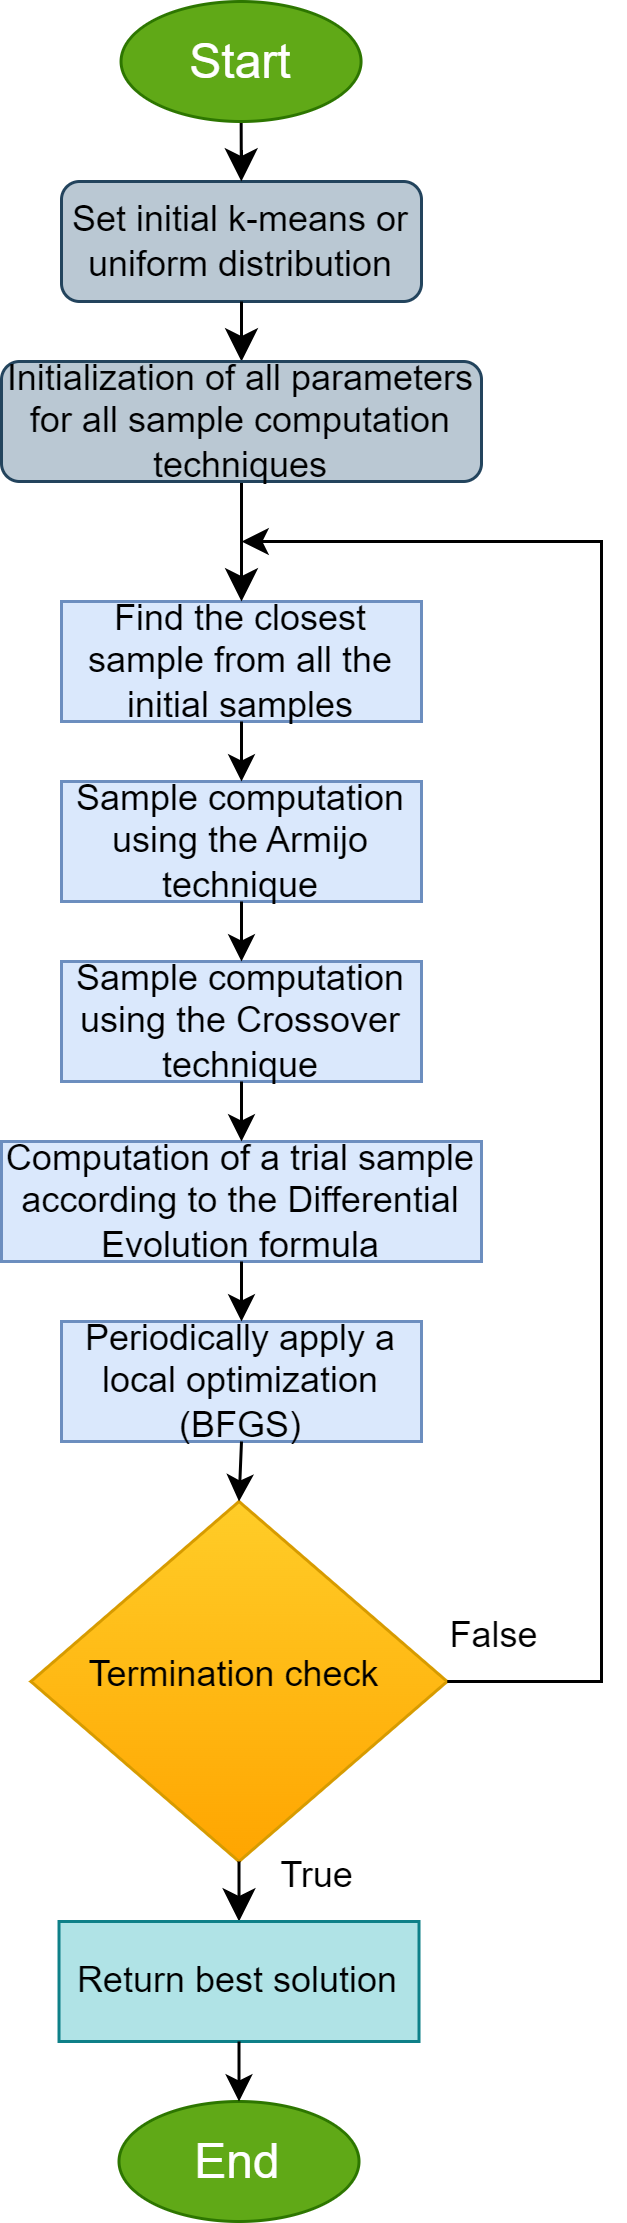
\includegraphics{hybridFlowChart}
\par\end{centering}
\caption{The flowchart of the proposed optimization procedure.\protect\label{fig:flow}}

\end{figure}

The optimization method described here combines evolutionary techniques,
such as differential evolution, Armijo line search, and components
of genetic algorithms, with the aim of finding the optimal solution.
Initially, the population size and the dimensionality of the target
function are defined, and the population samples are generated randomly
using a uniform or k-means distribution. For each sample, the Euclidean
distance (equation \ref{eq:nearestSamply}) to the other samples is
calculated to identify the nearest one, followed by an Armijo line
search (equation \ref{eq:findSample-1}) to determine the optimal
movement direction for the initial sample. Subsequently, a new offspring
sample is created using a crossover process (equation \ref{eq:makeChild}),
combining the current sample with the best discovered so far. A trial
vector (equation \ref{eq:trialSample}) is then formed, which accounts
for the adjustment of the computed samples and the differential coefficient
parameter derived from the differential evolution algorithm. Periodically,
local search methods, such as BFGS \citep{bfgs}, are applied to improve
the accuracy of the solution search. The method terminates when the
best solution found remains nearly unchanged for a specified number
of iterations. In summary, the basic steps for calculating a new sample
are:
\begin{itemize}
\item Identification of the nearest point \textbf{$c_{\iota}$ }for each
sample\textbf{ $x_{\iota}$}.
\item Calculation of a sample $\mbox{minLS}(x_{i},c_{i})$ through Armijo
line search, between the sample \textbf{$x_{i}$ }and the sample$c_{i}$.
\item Generation of the sample using the crossover process of the Genetic
Algorithm, between the sample \textbf{$x_{\iota}$ }and the best sample$x^{best}$
.
\item Computation of the trial point $y_{i}$ using a process derived from
Differential Evolution.
\end{itemize}

\section{Experiments\protect\label{sec:Experiments}}

\subsection{Settings and benchmark functions}

The benchmark functions used in the experimental measurements are
presented in Table \ref{tab:benchmarkFunctions}. 
\begin{table}[H]
\caption{The benchmark functions used in the conducted experiments.\protect\label{tab:benchmarkFunctions}}

\centering{}%
\begin{tabular}{|c|c|c|}
\hline 
{\footnotesize NAME} & {\scriptsize FORMULA} & {\scriptsize DIMENSION}\tabularnewline
\hline 
\hline 
{\footnotesize ACKLEY} & {\scriptsize$f(x)=-a\exp\left(-b\sqrt{\frac{1}{n}\sum_{i=1}^{n}x_{i}^{2}}\right)-\exp\left(\frac{1}{n}\sum_{i=1}^{n}\cos\left(cx_{i}\right)\right)+a+\exp(1)\quad a=20.0$} & {\scriptsize 2}\tabularnewline
\hline 
{\footnotesize BF1} & {\scriptsize$f(x)=-20\exp\left(-b\sqrt{\frac{1}{n}\sum_{i=1}^{n}x_{i}^{2}}\right)-\exp\left(\frac{1}{n}\sum_{i=1}^{n}\cos\left(cx_{i}\right)\right)+20+\exp(1)$} & {\scriptsize 2}\tabularnewline
\hline 
{\footnotesize BF1} & {\scriptsize$f(x)=x_{1}^{2}+2x_{2}^{2}-\frac{3}{10}\cos\left(3\pi x_{1}\right)-\frac{4}{10}\cos\left(4\pi x_{2}\right)+\frac{7}{10}$} & {\scriptsize 2}\tabularnewline
\hline 
{\footnotesize BF2} & {\scriptsize$f(x)=x_{1}^{2}+2x_{2}^{2}-\frac{3}{10}\cos\left(3\pi x_{1}\right)\cos\left(4\pi x_{2}\right)+\frac{3}{10}$} & {\scriptsize 2}\tabularnewline
\hline 
{\footnotesize BF3} & {\scriptsize$f(x)=x_{1}^{2}+2x_{2}^{2}-\frac{3}{10}\cos\left(3\pi x_{1}\right)\cos\left(4\pi x_{2}\right)+\frac{3}{10}$} & {\scriptsize 2}\tabularnewline
\hline 
{\footnotesize DIFFPOWER} & {\scriptsize$f(x)=\sum_{i=1}^{n}|x_{i}-y_{i}|^{p}$} & {\scriptsize$n=2\ p=2,5,10$}\tabularnewline
\hline 
{\footnotesize CAMEL} & {\scriptsize$f(x)=4x_{1}^{2}-2.1x_{1}^{4}+\frac{1}{3}x_{1}^{6}+x_{1}x_{2}-4x_{2}^{2}+4x_{2}^{4},\quad x\in[-5,5]^{2}$} & {\scriptsize 2}\tabularnewline
\hline 
{\footnotesize EASOM} & {\scriptsize$f(x)=-\cos\left(x_{1}\right)\cos\left(x_{2}\right)\exp\left(\left(x_{2}-\pi\right)^{2}-\left(x_{1}-\pi\right)^{2}\right)$} & {\scriptsize 2}\tabularnewline
\hline 
{\footnotesize ELP} & {\scriptsize$f(x)=\sum_{i=1}^{n}\left(10^{6}\right)^{\frac{i-1}{n-1}}x_{i}^{2}$} & {\scriptsize$n=10,20,30$}\tabularnewline
\hline 
{\footnotesize EXP} & {\scriptsize$f(x)=-\exp\left(-0.5\sum_{i=1}^{n}x_{i}^{2}\right),\quad-1\le x_{i}\le1$} & {\scriptsize$n=4,8,16,32$}\tabularnewline
\hline 
{\footnotesize F3} & {\scriptsize$f(x)=\left(e^{-2.0\log(2.0)\left(\frac{(x_{1}-0.08)}{0.854}\right)^{2}}\right)\left(\sin\left(5.0\pi\left(x_{1}^{\frac{3.0}{4.0}}-0.05\right)\right)\right)^{6}\quad x\in[0,1]^{n}$} & {\scriptsize 2}\tabularnewline
\hline 
{\footnotesize F5} & {\scriptsize$f(x)=\left(\left(4.0-2.1x_{1}^{2}+\frac{x_{1}^{4}}{3.0}\right)x_{1}^{2}\right)+\left(x_{1}x_{2}\right)+\left(\left(4.0x_{2}^{2}-4.0\right)x_{2}^{2}\right)\quad-5\le x_{i}\le5$} & {\scriptsize 2}\tabularnewline
\hline 
{\footnotesize F9} & {\scriptsize$f(x)=-\exp\left(-0.5\sum_{i=1}^{n}x_{i}^{2}\right),\quad x\in[0,1]^{n}$} & {\scriptsize 2}\tabularnewline
\hline 
{\footnotesize GKLS\citep{Gaviano}} & {\scriptsize$f(x)=\mbox{Gkls}(x,n,w)$} & {\scriptsize$n=2,3\ w=50,100$}\tabularnewline
\hline 
{\footnotesize GRIEWANK2} & {\scriptsize$f(x)=1+\frac{1}{200}\sum_{i=1}^{2}x_{i}^{2}-\prod_{i=1}^{2}\frac{\cos(x_{i})}{\sqrt{(i)}}$} & {\scriptsize 2}\tabularnewline
\hline 
{\footnotesize GRIEWANK10} & {\scriptsize f$(x)=1+\frac{1}{200}\sum_{i=1}^{10}x_{i}^{2}-\prod_{i=1}^{10}\frac{\cos(x_{i})}{\sqrt{(i)}}$} & {\scriptsize 10}\tabularnewline
\hline 
{\footnotesize HANSEN} & {\scriptsize$f(x)=\sum_{i=1}^{5}i\cos\left[(i-1)x_{1}+i\right]\sum_{j=1}^{5}j\cos\left[(j+1)x_{2}+j\right]$} & {\scriptsize 2}\tabularnewline
\hline 
{\footnotesize HARTMAN3} & {\scriptsize$f(x)=-\sum_{i=1}^{4}c_{i}\exp\left(-\sum_{j=1}^{3}a_{ij}\left(x_{j}-p_{ij}\right)^{2}\right)$} & {\scriptsize 3}\tabularnewline
\hline 
{\footnotesize HARTAMN6} & {\scriptsize$f(x)=-\sum_{i=1}^{4}c_{i}\exp\left(-\sum_{j=1}^{6}a_{ij}\left(x_{j}-p_{ij}\right)^{2}\right)$} & {\scriptsize 6}\tabularnewline
\hline 
{\footnotesize POTENTIAL\citep{Lennard}} & {\scriptsize$V_{LJ}(r)=4\epsilon\left[\left(\frac{\sigma}{r}\right)^{12}-\left(\frac{\sigma}{r}\right)^{6}\right]$} & {\scriptsize$n=9,15,21,30$}\tabularnewline
\hline 
{\footnotesize RARSTIGIN} & {\scriptsize$f(x)=x_{1}^{2}+x_{2}^{2}-\cos(18x_{1})-\cos(18x_{2})$} & {\scriptsize 2}\tabularnewline
\hline 
{\footnotesize ROSENBROCK} & {\tiny$f(x)=\sum_{i=1}^{n-1}\left(100\left(x_{i+1}-x_{i}^{2}\right)^{2}+\left(x_{i}-1\right)^{2}\right),\quad-30\le x_{i}\le30$} & {\scriptsize$n=4,8,16$}\tabularnewline
\hline 
{\footnotesize SCHWEFELH} & {\tiny$f(x)=\sum_{i=1}^{n}\left(\sum_{j=1}^{i}x_{j}\right)^{2}$} & {\scriptsize 2}\tabularnewline
\hline 
{\footnotesize SCHWEFELH221} & {\tiny$f(x)=418.9829n+\sum_{i=1}^{n}-x_{i}\sin\left(\sqrt{\left|x_{i}\right|}\right)$} & {\scriptsize 2}\tabularnewline
\hline 
{\footnotesize SCHWEFELH222} & {\tiny$f(x)=\sum_{i=1}^{n-1}\left(100\left(x_{i+1}-x_{i}^{2}\right)^{2}+\left(x_{i}-1\right)^{2}\right),\quad-30\le x_{i}\le30$} & {\scriptsize 2}\tabularnewline
\hline 
{\footnotesize Shekel5} & {\scriptsize$f(x)=-\sum_{i=1}^{5}\frac{1}{(x-a_{i})(x-a_{i})^{T}+c_{i}}$} & {\scriptsize 4}\tabularnewline
\hline 
{\footnotesize Shekel7} & {\scriptsize$f(x)=-\sum_{i=1}^{7}\frac{1}{(x-a_{i})(x-a_{i})^{T}+c_{i}}$} & {\scriptsize 4}\tabularnewline
\hline 
{\footnotesize Shekel10} & {\scriptsize$f(x)=-\sum_{i=1}^{10}\frac{1}{(x-a_{i})(x-a_{i})^{T}+c_{i}}$} & {\scriptsize 4}\tabularnewline
\hline 
{\footnotesize Sinusoidal\citep{Zabinsky}} & {\scriptsize$f(x)=-\left(2.5\prod_{i=1}^{n}\sin\left(x_{i}-z\right)+\prod_{i=1}^{n}\sin\left(5\left(x_{i}-z\right)\right)\right),\quad0\le x_{i}\le\pi$} & {\scriptsize$n=4,8$}\tabularnewline
\hline 
{\footnotesize Test2N} & {\scriptsize$f(x)=\frac{1}{2}\sum_{i=1}^{n}x_{i}^{4}-16x_{i}^{2}+5x_{i}$} & {\scriptsize$n=4,5,7$}\tabularnewline
\hline 
{\footnotesize Test30N} & {\scriptsize$\frac{1}{10}\sin^{2}\left(3\pi x_{1}\right)\sum_{i=2}^{n-1}\left(\left(x_{i}-1\right)^{2}\left(1+\sin^{2}\left(3\pi x_{i+1}\right)\right)\right)+\left(x_{n}-1\right)^{2}\left(1+\sin^{2}\left(2\pi x_{n}\right)\right)$} & {\scriptsize$n=3,4$}\tabularnewline
\hline 
\end{tabular}
\end{table}
 The functions used in the conducted experiments have been proposed
by various researchers \citep{Ali1,Floudas1} in the relevant literature.
For a more accurate comparison of the methods, efforts were made to
maintain certain parameter values at equal or similar levels. The
values for the parameters of the algorithm are presented in Table
\ref{tab:settings}, along with some explanation of each parameter.
\begin{center}
\begin{table}[H]
\caption{Parameters of optimization methods settings\protect\label{tab:settings}}

\centering{}%
\begin{tabular}{|c|c|c|}
\hline 
PARAMETER & VALUE & EXPLANATION\tabularnewline
\hline 
\hline 
$N$ & $200$ & Number of samples for all methods\tabularnewline
\hline 
$N_{k}$ & $200$ & Maximum number of iterations for all methods\tabularnewline
\hline 
$SR$ & $\left|f_{\mbox{min}}^{(k)}-f_{\mbox{min}}^{(k-1)}\right|$ & Best fitness: Stopping rule for all methods\tabularnewline
\hline 
$N_{t}$ & $12$ & Similarity max count for all methods\tabularnewline
\hline 
$LS$ & $0.05$\ $(5\%)$ & Local search rate for all methods\tabularnewline
\hline 
$F$ & $0.8$ & Differential weight for Differential Evolution\tabularnewline
\hline 
$CR$ & $0.9$ & Crossover Probability for Differential Evolution\tabularnewline
\hline 
$C_{1},C_{2}$ & $0.5$ & Parameters of PSO\tabularnewline
\hline 
$G_{c}$ & $0.1$\ $(10\%)$ & Crossover rate for Genetic Algorithm\tabularnewline
\hline 
$G_{m}$ & $0.05$\ $(5\%)$ & Mutation rate for Genetic Algorithm\tabularnewline
\hline 
$M_{k}$ & $10$ & Number of samples of sub-population for MEWOA \tabularnewline
\hline 
$M_{r}$ & $1$ & Number of iterations of exchange information for MEWOA\tabularnewline
\hline 
\end{tabular}
\end{table}
\par\end{center}

\subsection{Experimental results}

In the random number generator, different seeds were used to ensure
the reliability of the experimental results, with the experiments
being repeated 30 times. This process of repetition aims to minimize
the likelihood of random errors and to enhance the validity of the
results. The experiments were conducted on a system with an AMD Ryzen
5950X processor and 128 GB of RAM, operating in a Linux-Debian environment.
Additionally, the open-source optimizer \textquotedbl GlobalOptimus\textquotedbl{}
was used, which is a fully developed optimizer and is available for
distribution via the link: \url{http://www.github.com/itsoulos/GlobalOptimus}
(accessed on 7 November 2024). This optimization software can be installed
in any operating system (Linux, Windows, FreeBsd) when the Qt library
is available. The software includes a variety of optimization methods
as swll as some scripts to automate the optimization process under
Windows or Linux. Also, the software provides a graphical user interface
under the name Xoptimus and an installation file without dependencies
for Windows system is also included. In Table \ref{tab:mainTable},
the average function calls for each method and every objective function
is presented. The following notation is used in the experimental tables:
\begin{enumerate}
\item The column FUNCTION represents the name of the used objective problem.
\item The column GENETIC represents the application of the Genetic Algorithm
to the objective problem \citep{genetic3}.
\item The PSO column represents the implementation of the classical PSO
algorithm as suggested by the literature \citep{pso_major}.
\item The column IPSO stands for the application of the Improved PSO algorithm
as suggested by Charilogis and Tsoulos \citep{charilogis} to the
objective problems.
\item The column DE represents the average function calls for the Differential
Evolution optimization technique \citep{key-6}.
\item The column GWO represents the average function calls for the Gray
Wolf optimization technique \citep{gwo}.
\item The column WOA represents the average function calls for the Whale
Optimization technique \citep{WOA}.
\item The column MEWOA stands for the application of the Improved WOA algorithm
as suggested by Shen Y. et al \citep{memoa} to the objective problems.
\item The total sum of calls for each method is listed at the end of the
table. 
\item The column PROPOSED stands for the application of the current method.
\item The column KMEANS denotes the incorporation of KMEANS sampling in
the current method.
\end{enumerate}
{\footnotesize{}
\begin{table}[H]
\begin{centering}
{\footnotesize\caption{Comparison of average function calls of proposed method against others\protect\label{tab:mainTable}}
}{\footnotesize\par}
\par\end{centering}
{\scriptsize{}%
\begin{tabular}{|c|c|c|c|c|c|c|c|c|c|}
\hline 
{\scriptsize FUNCTION} & {\scriptsize GEN} & {\scriptsize PSO} & {\scriptsize IPSO} & {\scriptsize DE} & {\scriptsize GWO} & {\scriptsize WOA} & {\scriptsize MEWOA} & {\scriptsize PROPOSED} & {\scriptsize KMEANS}\tabularnewline
\hline 
\hline 
{\scriptsize ACKLEY} & {\scriptsize 6749} & {\scriptsize 6885} & {\scriptsize 3418} & {\scriptsize 16183} & {\scriptsize 20182} & {\scriptsize 24766} & {\scriptsize 13879} & {\scriptsize 5818} & {\scriptsize 3490}\tabularnewline
\hline 
{\scriptsize BF1} & {\scriptsize 4007} & {\scriptsize 4113} & {\scriptsize 1814} & {\scriptsize 8268} & {\scriptsize 9120} & {\scriptsize 9924} & {\scriptsize 7987} & {\scriptsize 5585} & {\scriptsize 3023}\tabularnewline
\hline 
{\scriptsize BF2} & {\scriptsize 3793} & {\scriptsize 3747} & {\scriptsize 1759} & {\scriptsize 7913} & {\scriptsize 8731} & {\scriptsize 9597} & {\scriptsize 6262} & {\scriptsize 5008} & {\scriptsize 2693}\tabularnewline
\hline 
{\scriptsize BF3} & {\scriptsize 3479} & {\scriptsize 3305} & {\scriptsize 1689} & {\scriptsize 6327} & {\scriptsize 7791} & {\scriptsize 20117} & {\scriptsize 5893} & {\scriptsize 4282} & {\scriptsize 2442}\tabularnewline
\hline 
{\scriptsize BRANIN} & {\scriptsize 2376} & {\scriptsize 2522} & {\scriptsize 1730} & {\scriptsize 4101} & {\scriptsize 6055} & {\scriptsize 5939} & {\scriptsize 3367} & {\scriptsize 3026} & {\scriptsize 2087}\tabularnewline
\hline 
{\scriptsize CAMEL} & {\scriptsize 2869} & {\scriptsize 2908} & {\scriptsize 1754} & {\scriptsize 5609} & {\scriptsize 6688} & {\scriptsize 5917} & {\scriptsize 4756} & {\scriptsize 3327} & {\scriptsize 2607}\tabularnewline
\hline 
{\scriptsize DIFFPOWER2} & {\scriptsize 5443} & {\scriptsize 8657} & {\scriptsize 2462} & {\scriptsize 14669} & {\scriptsize 22059} & {\scriptsize 11436} & {\scriptsize 11536} & {\scriptsize 8864} & {\scriptsize 5617}\tabularnewline
\hline 
{\scriptsize DIFFPOWER5} & {\scriptsize 18552} & {\scriptsize 24894} & {\scriptsize 4446} & {\scriptsize 39018} & {\scriptsize 49769} & {\scriptsize 42095} & {\scriptsize 31372} & {\scriptsize 26065} & {\scriptsize 17221}\tabularnewline
\hline 
{\scriptsize DIFFPOWER10} & {\scriptsize 18801} & {\scriptsize 32534} & {\scriptsize 4690} & {\scriptsize 46914} & {\scriptsize 54442} & {\scriptsize 56381} & {\scriptsize 38559} & {\scriptsize 29549} & {\scriptsize 26615}\tabularnewline
\hline 
{\scriptsize EASOM} & {\scriptsize 1958} & {\scriptsize 1998} & {\scriptsize 1753} & {\scriptsize 2978} & {\scriptsize 4615} & {\scriptsize 3153} & {\scriptsize 2455} & {\scriptsize 2755} & {\scriptsize 1402}\tabularnewline
\hline 
{\scriptsize ELP10} & {\scriptsize 3131} & {\scriptsize 4397} & {\scriptsize 1720} & {\scriptsize 6288} & {\scriptsize 9415} & {\scriptsize 10317} & {\scriptsize 5255} & {\scriptsize 4020} & {\scriptsize 3593}\tabularnewline
\hline 
{\scriptsize ELP20} & {\scriptsize 6160} & {\scriptsize 6883} & {\scriptsize 1988} & {\scriptsize 10794} & {\scriptsize 14173} & {\scriptsize 17040} & {\scriptsize 7722} & {\scriptsize 6537} & {\scriptsize 6194}\tabularnewline
\hline 
{\scriptsize ELP30} & {\scriptsize 9576} & {\scriptsize 9438} & {\scriptsize 2100} & {\scriptsize 14172} & {\scriptsize 18245} & {\scriptsize 23532} & {\scriptsize 9776} & {\scriptsize 8270} & {\scriptsize 3593}\tabularnewline
\hline 
{\scriptsize EXP4} & {\scriptsize 2946} & {\scriptsize 3177} & {\scriptsize 1677} & {\scriptsize 5166} & {\scriptsize 6648} & {\scriptsize 5567} & {\scriptsize 4392} & {\scriptsize 3570} & {\scriptsize 2238}\tabularnewline
\hline 
{\scriptsize EXP16} & {\scriptsize 3250} & {\scriptsize 3477} & {\scriptsize 1660} & {\scriptsize 6498} & {\scriptsize 6978} & {\scriptsize 9968} & {\scriptsize 4624} & {\scriptsize 3854} & {\scriptsize 3588}\tabularnewline
\hline 
{\scriptsize EXP32} & {\scriptsize 3561} & {\scriptsize 3728} & {\scriptsize 1647} & {\scriptsize 7606} & {\scriptsize 7419} & {\scriptsize 11925} & {\scriptsize 4508} & {\scriptsize 3852} & {\scriptsize 3691}\tabularnewline
\hline 
{\scriptsize F3} & {\scriptsize 4074} & {\scriptsize 3420} & {\scriptsize 1979} & {\scriptsize 7323} & {\scriptsize 10816} & {\scriptsize 11717} & {\scriptsize 5821} & {\scriptsize 6444} & {\scriptsize 5434}\tabularnewline
\hline 
{\scriptsize F5} & {\scriptsize 1630} & {\scriptsize 2055} & {\scriptsize 1376} & {\scriptsize 2814} & {\scriptsize 48377} & {\scriptsize 7393} & {\scriptsize 2117} & {\scriptsize 2697} & {\scriptsize 2199}\tabularnewline
\hline 
{\scriptsize F9} & {\scriptsize 2494} & {\scriptsize 2707} & {\scriptsize 1879} & {\scriptsize 4535} & {\scriptsize 5502} & {\scriptsize 4479} & {\scriptsize 3534} & {\scriptsize 4406} & {\scriptsize 1968}\tabularnewline
\hline 
{\scriptsize GKLS250} & {\scriptsize 2280} & {\scriptsize 2495} & {\scriptsize 1623} & {\scriptsize 3834} & {\scriptsize 6127} & {\scriptsize 4978} & {\scriptsize 3665} & {\scriptsize 2315} & {\scriptsize 1657}\tabularnewline
\hline 
{\scriptsize GKLS350} & {\scriptsize 2612} & {\scriptsize 2658} & {\scriptsize 1570} & {\scriptsize 3919} & {\scriptsize 6919} & {\scriptsize 7226} & {\scriptsize 3692} & {\scriptsize 2265} & {\scriptsize 1335}\tabularnewline
\hline 
{\scriptsize GOLDSTEIN} & {\scriptsize 3687} & {\scriptsize 3856} & {\scriptsize 1886} & {\scriptsize 6781} & {\scriptsize 9312} & {\scriptsize 9016} & {\scriptsize 5287} & {\scriptsize 3930} & {\scriptsize 2727}\tabularnewline
\hline 
{\scriptsize GRIEWANK2} & {\scriptsize 4500} & {\scriptsize 3168} & {\scriptsize 2299} & {\scriptsize 7429} & {\scriptsize 9253} & {\scriptsize 7948} & {\scriptsize 7285} & {\scriptsize 3850} & {\scriptsize 2223}\tabularnewline
\hline 
{\scriptsize GRIEWANK10} & {\scriptsize 6409} & {\scriptsize 7942} & {\scriptsize 2142} & {\scriptsize 18490} & {\scriptsize 14708} & {\scriptsize 51143} & {\scriptsize 12341} & {\scriptsize 7551} & {\scriptsize 6593}\tabularnewline
\hline 
{\scriptsize HANSEN} & {\scriptsize 3209} & {\scriptsize 2892} & {\scriptsize 2204} & {\scriptsize 4185} & {\scriptsize 7253} & {\scriptsize 10498} & {\scriptsize 4116} & {\scriptsize 4565} & {\scriptsize 3092}\tabularnewline
\hline 
{\scriptsize HARTMAN3} & {\scriptsize 2751} & {\scriptsize 3103} & {\scriptsize 1801} & {\scriptsize 5190} & {\scriptsize 7293} & {\scriptsize 8440} & {\scriptsize 3982} & {\scriptsize 3145} & {\scriptsize 2100}\tabularnewline
\hline 
{\scriptsize HARTMAN6} & {\scriptsize 3219} & {\scriptsize 3688} & {\scriptsize 1862} & {\scriptsize 5968} & {\scriptsize 8814} & {\scriptsize 22615} & {\scriptsize 4416} & {\scriptsize 4105} & {\scriptsize 2921}\tabularnewline
\hline 
{\scriptsize POTENTIAL3} & {\scriptsize 4351} & {\scriptsize 5154} & {\scriptsize 3096} & {\scriptsize 6218} & {\scriptsize 11256} & {\scriptsize 9232} & {\scriptsize 5071} & {\scriptsize 4790} & {\scriptsize 4034}\tabularnewline
\hline 
{\scriptsize POTENTIAL5} & {\scriptsize 7704} & {\scriptsize 10128} & {\scriptsize 6353} & {\scriptsize 9119} & {\scriptsize 22136} & {\scriptsize 39455} & {\scriptsize 8807} & {\scriptsize 7995} & {\scriptsize 7991}\tabularnewline
\hline 
{\scriptsize POTENTIAL6} & {\scriptsize 10177} & {\scriptsize 11780} & {\scriptsize 7593} & {\scriptsize 10509} & {\scriptsize 32630} & {\scriptsize 46466} & {\scriptsize 11341} & {\scriptsize 8906} & {\scriptsize 9333}\tabularnewline
\hline 
{\scriptsize POTENTIAL10} & {\scriptsize 13357} & {\scriptsize 16550} & {\scriptsize 10413} & {\scriptsize 12721} & {\scriptsize 38337} & {\scriptsize 59487} & {\scriptsize 18573} & {\scriptsize 12757} & {\scriptsize 13611}\tabularnewline
\hline 
{\scriptsize RASTRIGIN} & {\scriptsize 4106} & {\scriptsize 3539} & {\scriptsize 2211} & {\scriptsize 6216} & {\scriptsize 9043} & {\scriptsize 8116} & {\scriptsize 5523} & {\scriptsize 3672} & {\scriptsize 2364}\tabularnewline
\hline 
{\scriptsize ROSENBROCK4} & {\scriptsize 3679} & {\scriptsize 5858} & {\scriptsize 2025} & {\scriptsize 8452} & {\scriptsize 8078} & {\scriptsize 10759} & {\scriptsize 7750} & {\scriptsize 5642} & {\scriptsize 3641}\tabularnewline
\hline 
{\scriptsize ROSENBROCK8} & {\scriptsize 5269} & {\scriptsize 7843} & {\scriptsize 2085} & {\scriptsize 11530} & {\scriptsize 11167} & {\scriptsize 14094} & {\scriptsize 9469} & {\scriptsize 7926} & {\scriptsize 6119}\tabularnewline
\hline 
{\scriptsize ROSENBROCK16} & {\scriptsize 8509} & {\scriptsize 11450} & {\scriptsize 2432} & {\scriptsize 17432} & {\scriptsize 15590} & {\scriptsize 23544} & {\scriptsize 13554} & {\scriptsize 11285} & {\scriptsize 7490}\tabularnewline
\hline 
{\scriptsize SCHWEFEL} & {\scriptsize 1880} & {\scriptsize 2178} & {\scriptsize 1504} & {\scriptsize 3437} & {\scriptsize 4564} & {\scriptsize 4158} & {\scriptsize 3005} & {\scriptsize 2208} & {\scriptsize 1572}\tabularnewline
\hline 
{\scriptsize SCHWEFEL221} & {\scriptsize 2666} & {\scriptsize 2529} & {\scriptsize 1875} & {\scriptsize 3909} & {\scriptsize 71847} & {\scriptsize 8519} & {\scriptsize 3815} & {\scriptsize 2867} & {\scriptsize 2256}\tabularnewline
\hline 
{\scriptsize SCHWEFEL222} & {\scriptsize 33724} & {\scriptsize 42897} & {\scriptsize 28965} & {\scriptsize 86861} & {\scriptsize 101960} & {\scriptsize 114161} & {\scriptsize 65835} & {\scriptsize 78734} & {\scriptsize 18058}\tabularnewline
\hline 
{\scriptsize SHEKEL5} & {\scriptsize 3325} & {\scriptsize 3886} & {\scriptsize 2018} & {\scriptsize 6662} & {\scriptsize 10043} & {\scriptsize 17010} & {\scriptsize 5359} & {\scriptsize 5322} & {\scriptsize 2657}\tabularnewline
\hline 
{\scriptsize SHEKEL7} & {\scriptsize 3360} & {\scriptsize 4009} & {\scriptsize 1994} & {\scriptsize 6967} & {\scriptsize 10079} & {\scriptsize 17873} & {\scriptsize 5344} & {\scriptsize 5503} & {\scriptsize 2648}\tabularnewline
\hline 
{\scriptsize SHEKEL10} & {\scriptsize 2488} & {\scriptsize 3985} & {\scriptsize 1914} & {\scriptsize 6757} & {\scriptsize 10055} & {\scriptsize 15524} & {\scriptsize 5321} & {\scriptsize 4784} & {\scriptsize 2901}\tabularnewline
\hline 
{\scriptsize SINU4} & {\scriptsize 2990} & {\scriptsize 3409} & {\scriptsize 1961} & {\scriptsize 5953} & {\scriptsize 8132} & {\scriptsize 10150} & {\scriptsize 4874} & {\scriptsize 3446} & {\scriptsize 2254}\tabularnewline
\hline 
{\scriptsize SINU8} & {\scriptsize 3441} & {\scriptsize 3995} & {\scriptsize 1853} & {\scriptsize 6973} & {\scriptsize 10481} & {\scriptsize 20782} & {\scriptsize 5586} & {\scriptsize 4371} & {\scriptsize 3359}\tabularnewline
\hline 
{\scriptsize SINU16} & {\scriptsize 4320} & {\scriptsize 4680} & {\scriptsize 2251} & {\scriptsize 6979} & {\scriptsize 15356} & {\scriptsize 34409} & {\scriptsize 7274} & {\scriptsize 6450} & {\scriptsize 5992}\tabularnewline
\hline 
{\scriptsize TEST2N4} & {\scriptsize 3330} & {\scriptsize 3390} & {\scriptsize 1930} & {\scriptsize 6396} & {\scriptsize 8093} & {\scriptsize 11876} & {\scriptsize 4930} & {\scriptsize 3569} & {\scriptsize 2204}\tabularnewline
\hline 
{\scriptsize TEST2N5} & {\scriptsize 4000} & {\scriptsize 3604} & {\scriptsize 1982} & {\scriptsize 6271} & {\scriptsize 8812} & {\scriptsize 16256} & {\scriptsize 5045} & {\scriptsize 3877} & {\scriptsize 2575}\tabularnewline
\hline 
{\scriptsize TEST2N7} & {\scriptsize 4775} & {\scriptsize 4020} & {\scriptsize 2157} & {\scriptsize 7074} & {\scriptsize 10124} & {\scriptsize 25005} & {\scriptsize 6363} & {\scriptsize 4285} & {\scriptsize 2831}\tabularnewline
\hline 
{\scriptsize TEST30N3} & {\scriptsize 3210} & {\scriptsize 4018} & {\scriptsize 2432} & {\scriptsize 6178} & {\scriptsize 7647} & {\scriptsize 8163} & {\scriptsize 5311} & {\scriptsize 4215} & {\scriptsize 4389}\tabularnewline
\hline 
{\scriptsize TEST30N4} & {\scriptsize 3678} & {\scriptsize 4504} & {\scriptsize 3354} & {\scriptsize 7006} & {\scriptsize 10656} & {\scriptsize 13596} & {\scriptsize 7069} & {\scriptsize 5013} & {\scriptsize 2901}\tabularnewline
\hline 
{\scriptsize\textbf{\textcolor{red}{TOTAL}}} & {\scriptsize\textbf{\textcolor{red}{261106}}} & {\scriptsize\textbf{\textcolor{red}{317168}}} & {\scriptsize\textbf{\textcolor{red}{145908}}} & {\scriptsize\textbf{\textcolor{red}{506409}}} & {\scriptsize\textbf{\textcolor{red}{802608}}} & {\scriptsize\textbf{\textcolor{red}{916996}}} & {\scriptsize\textbf{\textcolor{red}{419939}}} & {\scriptsize\textbf{\textcolor{red}{361454}}} & {\scriptsize\textbf{\textcolor{red}{230033}}}\tabularnewline
\hline 
{\scriptsize\textcolor{red}{MAX}} & {\scriptsize\textbf{\textcolor{red}{33724}}} & {\scriptsize\textbf{\textcolor{red}{42897}}} & {\scriptsize\textbf{\textcolor{red}{28965}}} & {\scriptsize\textbf{\textcolor{red}{86861}}} & {\scriptsize\textbf{\textcolor{red}{101960}}} & {\scriptsize\textbf{\textcolor{red}{114161}}} & {\scriptsize\textbf{\textcolor{red}{65835}}} & {\scriptsize\textbf{\textcolor{red}{78734}}} & {\scriptsize\textbf{\textcolor{red}{26615}}}\tabularnewline
\hline 
{\scriptsize\textcolor{red}{MIN}} & {\scriptsize\textbf{\textcolor{red}{1630}}} & {\scriptsize\textbf{\textcolor{red}{1998}}} & {\scriptsize\textbf{\textcolor{red}{1376}}} & {\scriptsize\textbf{\textcolor{red}{2814}}} & {\scriptsize\textbf{\textcolor{red}{4564}}} & {\scriptsize\textbf{\textcolor{red}{3153}}} & {\scriptsize\textbf{\textcolor{red}{2117}}} & {\scriptsize\textbf{\textcolor{red}{2208}}} & {\scriptsize\textbf{\textcolor{red}{1335}}}\tabularnewline
\hline 
{\scriptsize\textcolor{red}{STDEV}} & {\scriptsize\textbf{\textcolor{red}{5517.7}}} & {\scriptsize\textbf{\textcolor{red}{7735.58}}} & {\scriptsize\textbf{\textcolor{red}{4121.63}}} & {\scriptsize\textbf{\textcolor{red}{13674.61}}} & {\scriptsize\textbf{\textcolor{red}{18893.71}}} & {\scriptsize\textbf{\textcolor{red}{19622.90}}} & {\scriptsize\textbf{\textcolor{red}{10608.07}}} & {\scriptsize\textbf{\textcolor{red}{11562.76}}} & {\scriptsize\textbf{\textcolor{red}{5885.97}}}\tabularnewline
\hline 
{\scriptsize\textbf{\textcolor{red}{AVERAGE}}} & {\scriptsize\textbf{\textcolor{red}{5466.43}}} & {\scriptsize\textbf{\textcolor{red}{6613.33}}} & {\scriptsize\textbf{\textcolor{red}{3047.47}}} & {\scriptsize\textbf{\textcolor{red}{10665.14}}} & {\scriptsize\textbf{\textcolor{red}{16791.63}}} & {\scriptsize\textbf{\textcolor{red}{19219.63}}} & {\scriptsize\textbf{\textcolor{red}{8853.43}}} & {\scriptsize\textbf{\textcolor{red}{7495.35}}} & {\scriptsize\textbf{\textcolor{red}{5316.8}}}\tabularnewline
\hline 
{\scriptsize\textbf{\textcolor{red}{MEDIAN}}} & {\scriptsize\textbf{\textcolor{red}{3678}}} & {\scriptsize\textbf{\textcolor{red}{3886}}} & {\scriptsize\textbf{\textcolor{red}{1982}}} & {\scriptsize\textbf{\textcolor{red}{6781}}} & {\scriptsize\textbf{\textcolor{red}{9415}}} & {\scriptsize\textbf{\textcolor{red}{11717}}} & {\scriptsize\textbf{\textcolor{red}{5359}}} & {\scriptsize\textbf{\textcolor{red}{4406}}} & {\scriptsize\textbf{\textcolor{red}{2921}}}\tabularnewline
\hline 
{\scriptsize\textbf{\textcolor{red}{SKEW}}} & {\scriptsize\textbf{\textcolor{red}{3.54}}} & {\scriptsize\textbf{\textcolor{red}{3.35}}} & {\scriptsize\textbf{\textcolor{red}{5.55}}} & {\scriptsize\textbf{\textcolor{red}{4.32}}} & {\scriptsize\textbf{\textcolor{red}{2.89}}} & {\scriptsize\textbf{\textcolor{red}{2.9}}} & {\scriptsize\textbf{\textcolor{red}{4.02}}} & {\scriptsize\textbf{\textcolor{red}{5.3}}} & {\scriptsize\textbf{\textcolor{red}{2.53}}}\tabularnewline
\hline 
{\scriptsize\textbf{\textcolor{red}{KURT}}} & {\scriptsize\textbf{\textcolor{red}{14.75}}} & {\scriptsize\textbf{\textcolor{red}{12.05}}} & {\scriptsize\textbf{\textcolor{red}{34.01}}} & {\scriptsize\textbf{\textcolor{red}{21.19}}} & {\scriptsize\textbf{\textcolor{red}{9.12}}} & {\scriptsize\textbf{\textcolor{red}{10.87}}} & {\scriptsize\textbf{\textcolor{red}{18.43}}} & {\scriptsize\textbf{\textcolor{red}{31.3}}} & {\scriptsize\textbf{\textcolor{red}{5.77}}}\tabularnewline
\hline 
\end{tabular}}{\scriptsize\par}
\end{table}
}{\footnotesize\par}

\begin{table}[H]
\begin{centering}
\caption{Function calls with different differential weight F\protect\label{tab:differentF}}
\begin{tabular}{|c|c|c|c|}
\hline 
FUNCTION & Proposed(F:random) & Proposed (F:0.5) & Proposed (F:0.9)\tabularnewline
\hline 
\hline 
ACKLEY & 5818 & 5206 & 5379\tabularnewline
\hline 
BF1 & 5585 & 5797 & 5575\tabularnewline
\hline 
BF2 & 5008 & 4666 & 4734\tabularnewline
\hline 
BF3 & 4282 & 4309 & 4077\tabularnewline
\hline 
BRANIN & 3026 & 3078 & 2858\tabularnewline
\hline 
CAMEL & 3327 & 3253 & 3203\tabularnewline
\hline 
DIFFPOWER2 & 8864 & 8833 & 8834\tabularnewline
\hline 
DIFFPOWER5 & 26065 & 26067 & 26059\tabularnewline
\hline 
DIFFPOWER10 & 29549 & 29548 & 29537\tabularnewline
\hline 
EASOM & 2755 & 2668 & 2637\tabularnewline
\hline 
ELP10 & 4020 & 4020 & 4020\tabularnewline
\hline 
ELP20 & 6537 & 6537 & 6537\tabularnewline
\hline 
ELP30 & 8270 & 8270 & 8270\tabularnewline
\hline 
EXP4 & 3570 & 3570 & 3570\tabularnewline
\hline 
EXP16 & 3854 & 3854 & 3854\tabularnewline
\hline 
EXP32 & 3852 & 3852 & 3852\tabularnewline
\hline 
F1 & 6444 & 5649 & 5617\tabularnewline
\hline 
F5 & 2697 & 2551 & 2328\tabularnewline
\hline 
F9 & 4406 & 4063 & 3500\tabularnewline
\hline 
GKLS250 & 2315 & 2321 & 2316\tabularnewline
\hline 
GKLS350 & 2265(96) & 2244(90) & 2204(90)\tabularnewline
\hline 
GOLDSTEIN & 3930 & 3848 & 3917\tabularnewline
\hline 
GRIEWANK2 & 3850(50) & 3963(50) & 4052(50)\tabularnewline
\hline 
GRIEWANK10 & 7551 & 7551 & 7551\tabularnewline
\hline 
HANSEN & 4565 & 4187 & 3548\tabularnewline
\hline 
HARTMAN3 & 3145 & 3142 & 3139\tabularnewline
\hline 
HARTMAN6 & 4105 & 4070 & 4001\tabularnewline
\hline 
POTENTIAL3 & 4790 & 4653 & 4699\tabularnewline
\hline 
POTENTIAL5 & 7995 & 7987 & 7690\tabularnewline
\hline 
POTENTIAL6 & 8906(76) & 8926(70) & 8936(70)\tabularnewline
\hline 
POTENTIAL10 & 12757 & 12457 & 12452\tabularnewline
\hline 
RASTRIGIN & 3672(86) & 3358(80) & 3206(86)\tabularnewline
\hline 
ROSENBROCK4 & 5642 & 5641 & 5641\tabularnewline
\hline 
ROSENBROCK8 & 7926 & 7926 & 7926\tabularnewline
\hline 
ROSENBROCK16 & 11285 & 11285 & 11285\tabularnewline
\hline 
SCHWEFEL & 2208 & 2208 & 2208\tabularnewline
\hline 
SCHWEFEL221 & 2867 & 2858 & 2742\tabularnewline
\hline 
SCHWEFEL222 & 78734 & 89919 & 90250\tabularnewline
\hline 
SHEKEL5 & 5322 & 4721 & 4492\tabularnewline
\hline 
SHEKEL7 & 5503 & 4723 & 4666\tabularnewline
\hline 
SHEKEL10 & 4784 & 4385 & 4541\tabularnewline
\hline 
SINU4 & 3446 & 3634 & 3488\tabularnewline
\hline 
SINU8 & 4371 & 4373 & 4387\tabularnewline
\hline 
SINU16 & 6450 & 6543 & 6538\tabularnewline
\hline 
TEST2N4 & 3569 & 3487 & 3490\tabularnewline
\hline 
TEST2N5 & 3877(93) & 3704(96) & 3712(96)\tabularnewline
\hline 
TEST2N7 & 4285(50) & 4043(50) & 4190(53)\tabularnewline
\hline 
TEST30N3 & 4215 & 3412 & 3685\tabularnewline
\hline 
TEST30N4 & 5013 & 4812 & 4515\tabularnewline
\hline 
SUM & 361454 & 366966 & 342529\tabularnewline
\hline 
\end{tabular}
\par\end{centering}
\end{table}

\begin{table}[H]

\begin{centering}
\caption{Function calls with different number of population\protect\label{tab:differentPopulation}}
\begin{tabular}{|c|c|c|c|}
\hline 
FUNCTION & \begin{cellvarwidth}[t]
\centering
Proposed

(population=200)
\end{cellvarwidth} & \begin{cellvarwidth}[t]
\centering
Proposed

(population=150)
\end{cellvarwidth} & \begin{cellvarwidth}[t]
\centering
Proposed

(population=100)
\end{cellvarwidth}\tabularnewline
\hline 
\hline 
ACKLAY & 5818 & 4647 & 2829\tabularnewline
\hline 
BF1 & 5585 & 4303 & 2847\tabularnewline
\hline 
BF2 & 5008 & 3502 & 2334\tabularnewline
\hline 
BF3 & 4282 & 3034 & 2045\tabularnewline
\hline 
BRANIN & 3026 & 2300 & 1506\tabularnewline
\hline 
CAMEL & 3327 & 2526 & 1795\tabularnewline
\hline 
DIFFPOWER2 & 8864 & 6326 & 4094\tabularnewline
\hline 
DIFFPOWER5 & 26065 & 19239 & 14008\tabularnewline
\hline 
DIFFPOWER10 & 29549 & 22112 & 15325\tabularnewline
\hline 
EASOM & 2755 & 1976 & 1306\tabularnewline
\hline 
ELP10 & 4020 & 3080 & 2111\tabularnewline
\hline 
ELP20 & 6537 & 5080 & 3234\tabularnewline
\hline 
ELP30 & 8270 & 6300 & 4307\tabularnewline
\hline 
EXP4 & 3570 & 2718 & 1906\tabularnewline
\hline 
EXP16 & 3854 & 2938 & 1990\tabularnewline
\hline 
EXP32 & 3852 & 2700 & 1904\tabularnewline
\hline 
F1 & 6444 & 5232 & 3404\tabularnewline
\hline 
F5 & 2697 & 2100 & 1822\tabularnewline
\hline 
F9 & 4406 & 2999 & 2111\tabularnewline
\hline 
GKLS250 & 2315 & 1767 & 1191\tabularnewline
\hline 
GKLS350 & 2265(96) & 1699 (90) & 1050(60)\tabularnewline
\hline 
GOLDSTEIN & 3930 & 2826 & 1949\tabularnewline
\hline 
GRIEWANK2 & 3850(50) & 2803(56) & 1883(30)\tabularnewline
\hline 
GRIEWANK10 & 7551 & 5821 & 3933\tabularnewline
\hline 
HANSEN & 4565 & 2965 & 2024\tabularnewline
\hline 
HARTMAN3 & 3145 & 2440 & 1613\tabularnewline
\hline 
HARTMAN6 & 4105 & 3036 & 2004\tabularnewline
\hline 
POTENTIAL3 & 4790 & 3655 & 2416\tabularnewline
\hline 
POTENTIAL5 & 7995 & 6710 & 4215\tabularnewline
\hline 
POTENTIAL6 & 8906(76) & 8246(70) & 4890(33)\tabularnewline
\hline 
POTENTIAL10 & 12757 & 10417 & 6598(86)\tabularnewline
\hline 
RASTRIGIN & 3672(86) & 2525(73) & 1728(56)\tabularnewline
\hline 
ROSENBROCK4 & 5642 & 4343 & 2995\tabularnewline
\hline 
ROSENBROCK8 & 7926 & 5953 & 4083\tabularnewline
\hline 
ROSENBROCK16 & 11285 & 8694 & 5922\tabularnewline
\hline 
SCHWEFEL & 2208 & 1728 & 1125\tabularnewline
\hline 
SCHWEFEL221 & 2867 & 2192 & 1516\tabularnewline
\hline 
SCHWEFEL222 & 78734 & 64540 & 30545\tabularnewline
\hline 
SHEKEL5 & 5322 & 3863 & 2407\tabularnewline
\hline 
SHEKEL7 & 5503 & 3568 & 2556\tabularnewline
\hline 
SHEKEL10 & 4784 & 3277 & 2374\tabularnewline
\hline 
SINU4 & 3446 & 2561 & 1858\tabularnewline
\hline 
SINU8 & 4371 & 3292 & 2258\tabularnewline
\hline 
SINU16 & 6450 & 5162 & 3386\tabularnewline
\hline 
TEST2N4 & 3569 & 2597 & 1988(86)\tabularnewline
\hline 
TEST2N5 & 3877(93) & 3130(96) & 1915(80)\tabularnewline
\hline 
TEST2N7 & 4285(50) & 3325(36) & 2089(33)\tabularnewline
\hline 
TEST30N3 & 4215 & 2756 & 1870\tabularnewline
\hline 
TEST30N4 & 5013 & 3768 & 2115\tabularnewline
\hline 
SUM & 361454 & 278124 & 174545\tabularnewline
\hline 
\end{tabular}
\par\end{centering}
\end{table}

At the end of every global optimization procedure, a BFGS variant
of Powell \citep{powell} is utilized to improve the discovered solution
and identify with certainty a local minimum.  Additionally, Figure
\ref{fig:proposedVSOthers} presents a statistical comparison between
the used optimization methods and the data provided from Table \ref{tab:mainTable}.

\begin{figure}[H]
\centering{}\subfloat[With outliers appearing\label{fig:CompWith}]{
\centering{}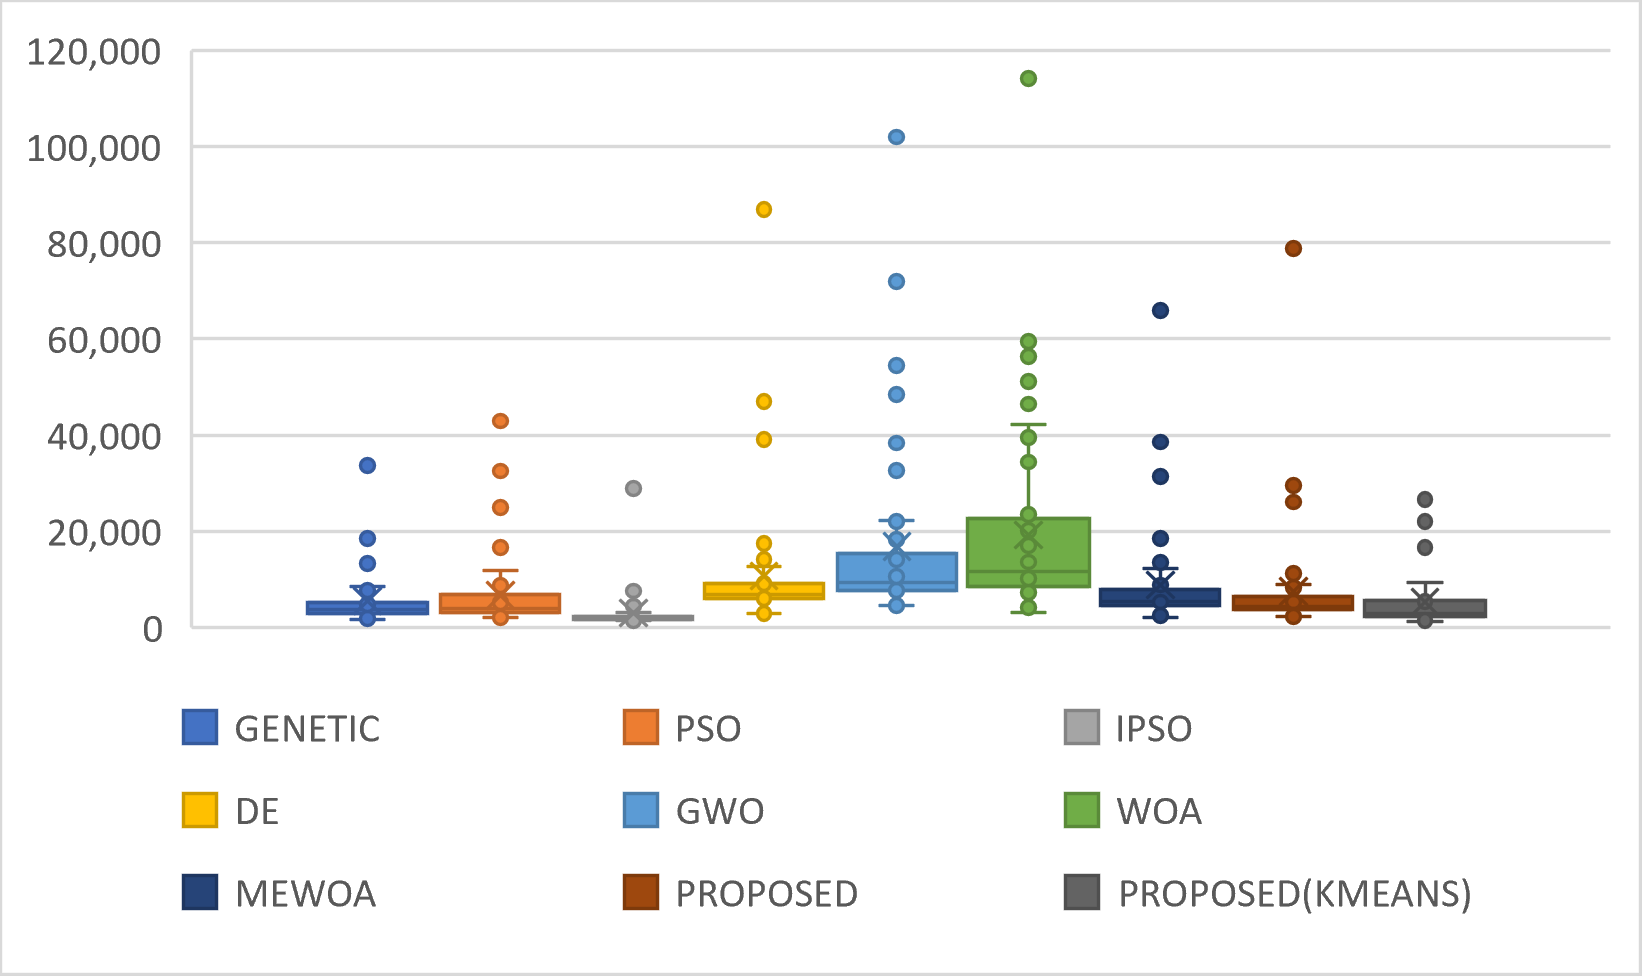
\includegraphics[scale=0.5]{new10}}\subfloat[Without outliers appearing\label{fig:CompWithout}]{\begin{centering}
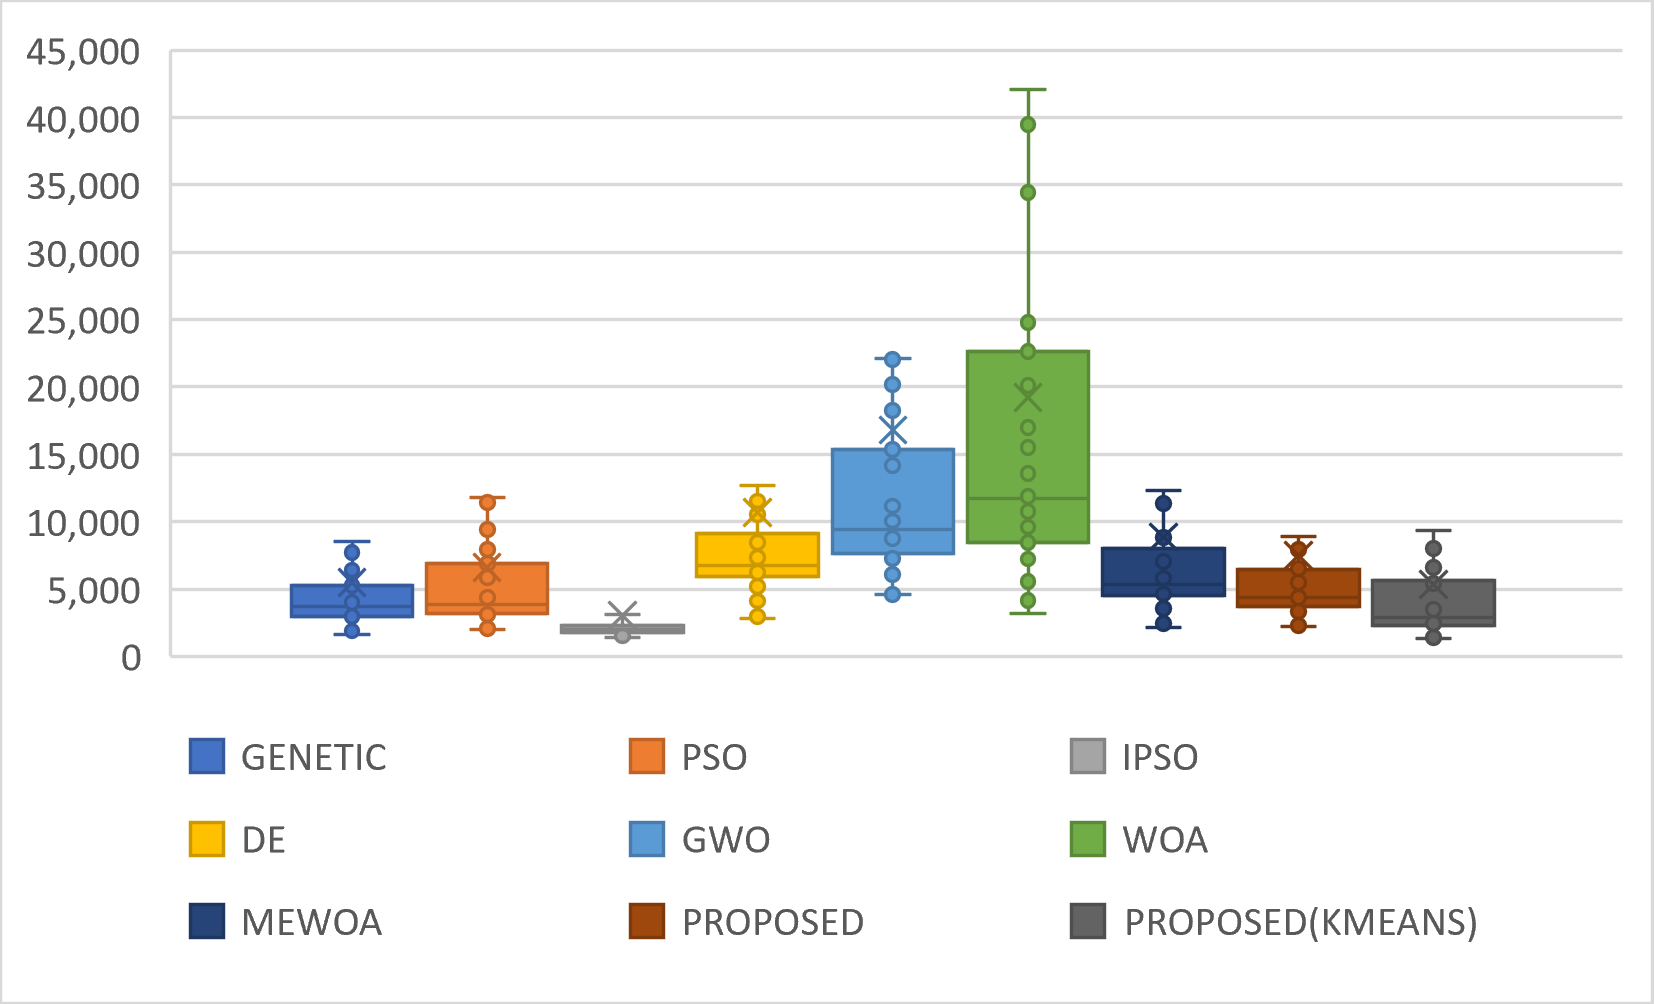
\includegraphics[scale=0.5]{new11}
\par\end{centering}
}\caption{Comparison using the number of function calls. The test was performed
for different optimization methods.\protect\label{fig:proposedVSOthers}}
\end{figure}
 

\begin{figure}[H]
\centering{}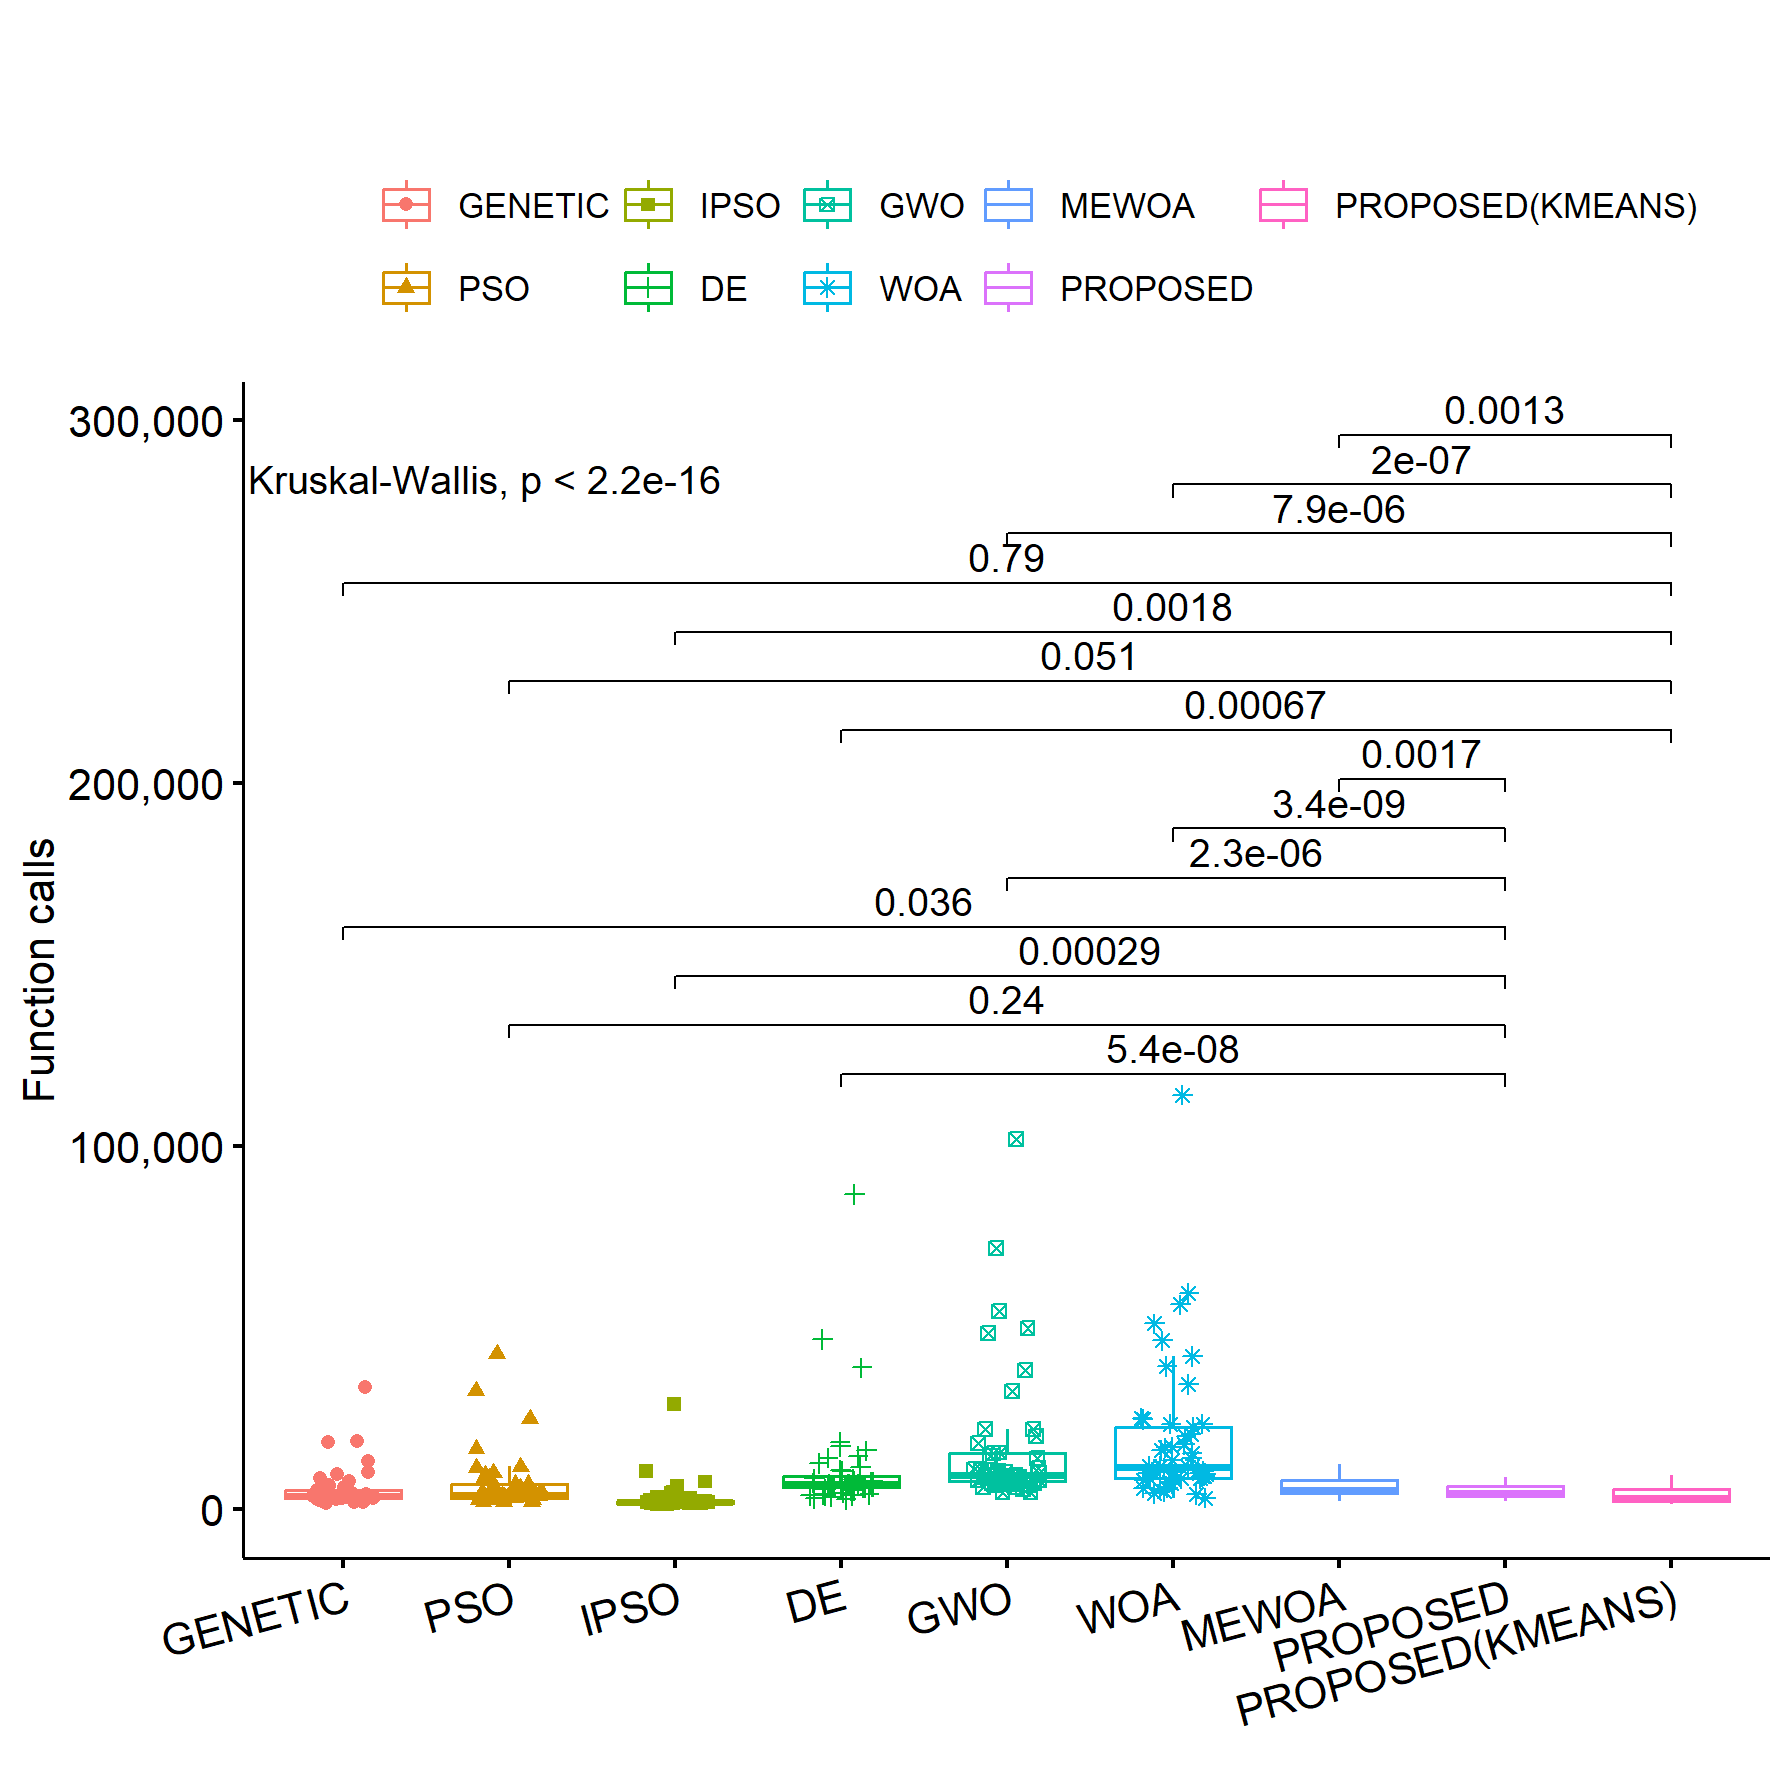
\includegraphics[scale=0.5]{new12}\caption{Statistical comparison of proposed method against others. The test
was performed for different optimization methods\protect\label{fig:StatProposedVSOthers}}
\end{figure}

The table \ref{tab:mainTable} contains values representing objective
function evaluations, with lower values indicating better performance.
The goal is to minimize the number of function calls required to achieve
a result. The algorithms analyzed are GENETIC, PSO, IPSO, DE, GWO,
WOA, MEWOA, PROPOSED, and PROPOSED(KMEANS). The GENETIC algorithm,
with a total of 261,106 evaluations, shows mixed results. In some
functions, such as SHEKEL10 with 2488 evaluations, it performs well.
However, in more demanding functions, like DIFFPOWER5 and DIFFPOWER10
with 18,552 and 18,801 evaluations respectively, it requires many
calls, indicating reduced efficiency. The PSO algorithm, with 317,168
total evaluations, needs more calls than GENETIC and is generally
considered less efficient. In difficult functions, such as DIFFPOWER10,
it requires many evaluations, indicating reduced effectiveness. The
IPSO algorithm is the most efficient, with only 145,908 evaluations.
Its low values in several functions, such as ROSENBROCK16 with 2432
calls and TEST2N5 with 1982 calls, indicate that it requires fewer
evaluations to achieve a result, making it the most efficient algorithm.
The DE algorithm, with 506,409 evaluations, performs worse compared
to IPSO and other algorithms. In difficult functions, such as DIFFPOWER10
with 46,914 calls and SCHWEFEL222 with 86,861 calls, it requires significantly
more evaluations, indicating difficulties in optimizing efficiently.
GWO has the most total evaluations (802,608), showing reduced efficiency.
It encounters particular difficulties in hard problems, such as DIFFPOWER10
with 54,442 calls and SCHWEFEL222 with 101,960 calls. WOA, with 916,996
evaluations, is even less efficient than GWO. It faces serious issues
in demanding functions such as DIFFPOWER10 (56,381 calls) and SCHWEFEL222
(114,161 calls), indicating poor performance. MEWOA (Modified WOA)
has 419,939 total evaluations, showing some improvement over WOA but
still less efficient than IPSO and PROPOSED+KMEANS. Despite the improvement,
it continues to require many calls in difficult problems, such as
DIFFPOWER10 (38,559 calls) and SCHWEFEL222 (65,835 calls). The PROPOSED
algorithm, with 361,454 evaluations, performs better than DE but does
not reach the efficiency of IPSO. It shows moderate results in some
problems, such as DIFFPOWER10 with 29,549 calls, limiting its overall
performance. The improved PROPOSED(KMEANS) algorithm achieves better
results, with 257,033 total evaluations. In many functions, such as
SCHWEFEL222 with 22,058 evaluations and DIFFPOWER10 with 26,615 evaluations,
the addition of KMEANS significantly improves performance, making
it competitive with IPSO. In conclusion, IPSO is the most efficient
algorithm, with the lowest total number of evaluations, achieving
better results with fewer calls. PROPOSED(KMEANS) also performs well,
approaching the performance of IPSO. On the other hand, GWO and WOA
have the worst performance, requiring the highest number of evaluations.
MEWOA shows some improvements over WOA but remains less efficient
than the top-performing algorithms.

In Figure \ref{fig:StatProposedVSOthers}, pairwise comparisons between
the proposed methods and the other methods are presented. In all these
comparisons, the critical parameter p<0.05 confirms the statistical
significance of the results.

Overall, the proposed methods achieve a significant reduction in the
required number of objective function calls and, in many cases, outperform
other optimization techniques. Compared to the Differential Evolution
(DE) algorithm, the proposed approaches perform better across all
mathematical models, with the reduction in the number of calls exceeding
50\%. This trend is confirmed by Table \ref{tab:mainTable}. Additionally,
Figures \ref{fig:CompWith}, \ref{fig:CompWithout}, and \ref{fig:StatProposedVSOthers}
present statistical comparisons between the global optimization methods
used in the experiments, highlighting the superiority of the proposed
approaches.

The table \ref{tab:differentF} presents the number of objective function
calls for different values of the differential weight F. When F is
randomly selected within the range {[}0.0, 1.0{]}, the total number
of calls is 361,454. With F=0.5, the calls increase to 366,966, while
with F=0.9, they decrease to 342,529, indicating the best performance.
This suggests that higher values of F improve convergence by reducing
the total function calls. Although random F values provide a good
balance between exploration and exploitation, they do not outperform
the fixed value F=0.9. On the other hand, F=0.5 appears to burden
the algorithm with more function calls. Therefore, selecting a higher
or adaptive F can enhance the algorithm’s efficiency by lowering computational
costs.

From the data in table \ref{tab:differentPopulation}, we observe
that as the population size decreases, the number of function calls
generally decreases as well, indicating increased efficiency with
smaller populations. For example, the ACKLAY function requires 5,818
calls with a population of 200, 4,647 with a population of 150, and
2,829 with a population of 100. A similar trend is seen with DIFFPOWER10,
which reduces from 29,549 to 22,112 and then to 15,325 as the population
size decreases. However, there is variation between functions. SCHWEFEL222
shows very high call numbers, particularly with a population of 200
(78,734 calls), suggesting increased complexity. In contrast, functions
like GKLS350 require fewer calls, even with larger populations. Although
calls often decrease with a smaller population, this does not necessarily
mean that the solution quality is maintained. Choosing the right population
size is crucial, as excessive reduction may limit the search space
and degrade optimization performance. Table \ref{tab:differentPopulation}
illustrates how population size impacts performance. Balancing population
size and the number of calls is essential for achieving efficient
and reliable results.

An additional experiment was executed for the High Elliptic function,
which is defined as:
\[
f(x)=\sum_{i=1}^{n}\left(10^{6}\right)^{\frac{i-1}{n-1}}x_{i}^{2}
\]
where the parameter $n$ defines the dimension of the function. In
this particular experiment, the proposed optimization method was systematically
applied to a specific mathematical function as the dimension $n$
underwent a transition from 10 to 100. Figure \ref{fig:ELPcalls}
presents the number of objective function calls required for each
algorithm across different dimensions. As the problem dimension increases,
the number of function calls needed to find a solution grows significantly
for all algorithms, indicating the increasing complexity of the ELP
function. For example, the PROPOSED(KMEANS) algorithm requires 3593
calls for 10 dimensions and 20,900 calls for 100 dimensions, showing
a gradual increase. Similarly, the PROPOSED algorithm starts with
4020 calls for 10 dimensions and reaches 24,322 calls for 100 dimensions.
IPSO stands out as the most efficient algorithm, with only 1720 calls
at 10 dimensions and 3165 at 100, consistently maintaining low evaluations.
In contrast, WOA exhibits the worst performance, with 10,317 calls
at 10 dimensions and 62,878 at 100 dimensions. The rate of increase
in calls varies among algorithms. For example, the PROPOSED algorithm
increases from 4020 to 6537 calls between 10 and 20 dimensions (a
1.6 times increase), while the rise from 90 to 100 dimensions is more
moderate, from 20,798 to 24,322 calls. MEWOA, although improved compared
to WOA, requires more calls than the proposed methods, with 5255 calls
at 10 dimensions and 26,684 at 100. GENETIC displays a variable pattern,
with 3131 calls at 10 dimensions and 29,004 at 100. GWO and PSO follow
a similar trend, with a gradual increase in calls as the dimension
increases. Additionally, Figure \ref{fig:ELPTimes} illustrates the
execution time for each algorithm across different dimensions, measured
in seconds. As expected, increasing the dimension leads to a significant
rise in execution time for all algorithms, highlighting the increased
computational load. For example, PROPOSED(KMEANS) starts with 0.652
seconds at 10 dimensions and reaches 23.54 seconds at 100. PROPOSED
begins with 0.236 seconds at 10 dimensions and climbs to 32.784 seconds
at 100, marking an impressive 139-fold increase. The fastest algorithm,
IPSO, takes only 0.034 seconds at 10 dimensions and 2.106 seconds
at 100, demonstrating excellent performance and scalability. On the
other hand, WOA records the worst performance, with 75.319 seconds
at 100 dimensions compared to 0.257 seconds at 10 dimensions. DE also
struggles in execution time, increasing from 0.16 seconds at 10 dimensions
to 47.68 seconds at 100. The increase in execution time across dimensions
follows a nonlinear trend for most algorithms. For example, PROPOSED
takes 0.587 seconds at 20 dimensions (more than double the 0.236 seconds
at 10 dimensions) but reaches 14.847 seconds at 80 dimensions. Similarly,
PSO starts at 0.128 seconds at 10 dimensions and reaches 20.361 seconds
at 100 dimensions. 

The data reveals significant differences in the scalability and efficiency
of the algorithms. IPSO stands out as the most efficient algorithm,
with the lowest number of calls and the shortest execution time. PROPOSED(KMEANS)
also achieves satisfactory results, maintaining a balance between
calls and execution time. On the other hand, WOA and GWO exhibit the
worst performance, with significantly more calls and substantial increases
in execution time as the dimension grows.

The results confirm that the complexity of optimization problems increases
sharply with the dimension. Most algorithms struggle to maintain their
efficiency in higher dimensions, highlighting the importance of selecting
the appropriate algorithm according to the problem's requirements
and the available computational resources.
\begin{center}
\begin{figure}[H]
\centering{}\subfloat[Comparison of the function calls\label{fig:ELPcalls}]{\centering{}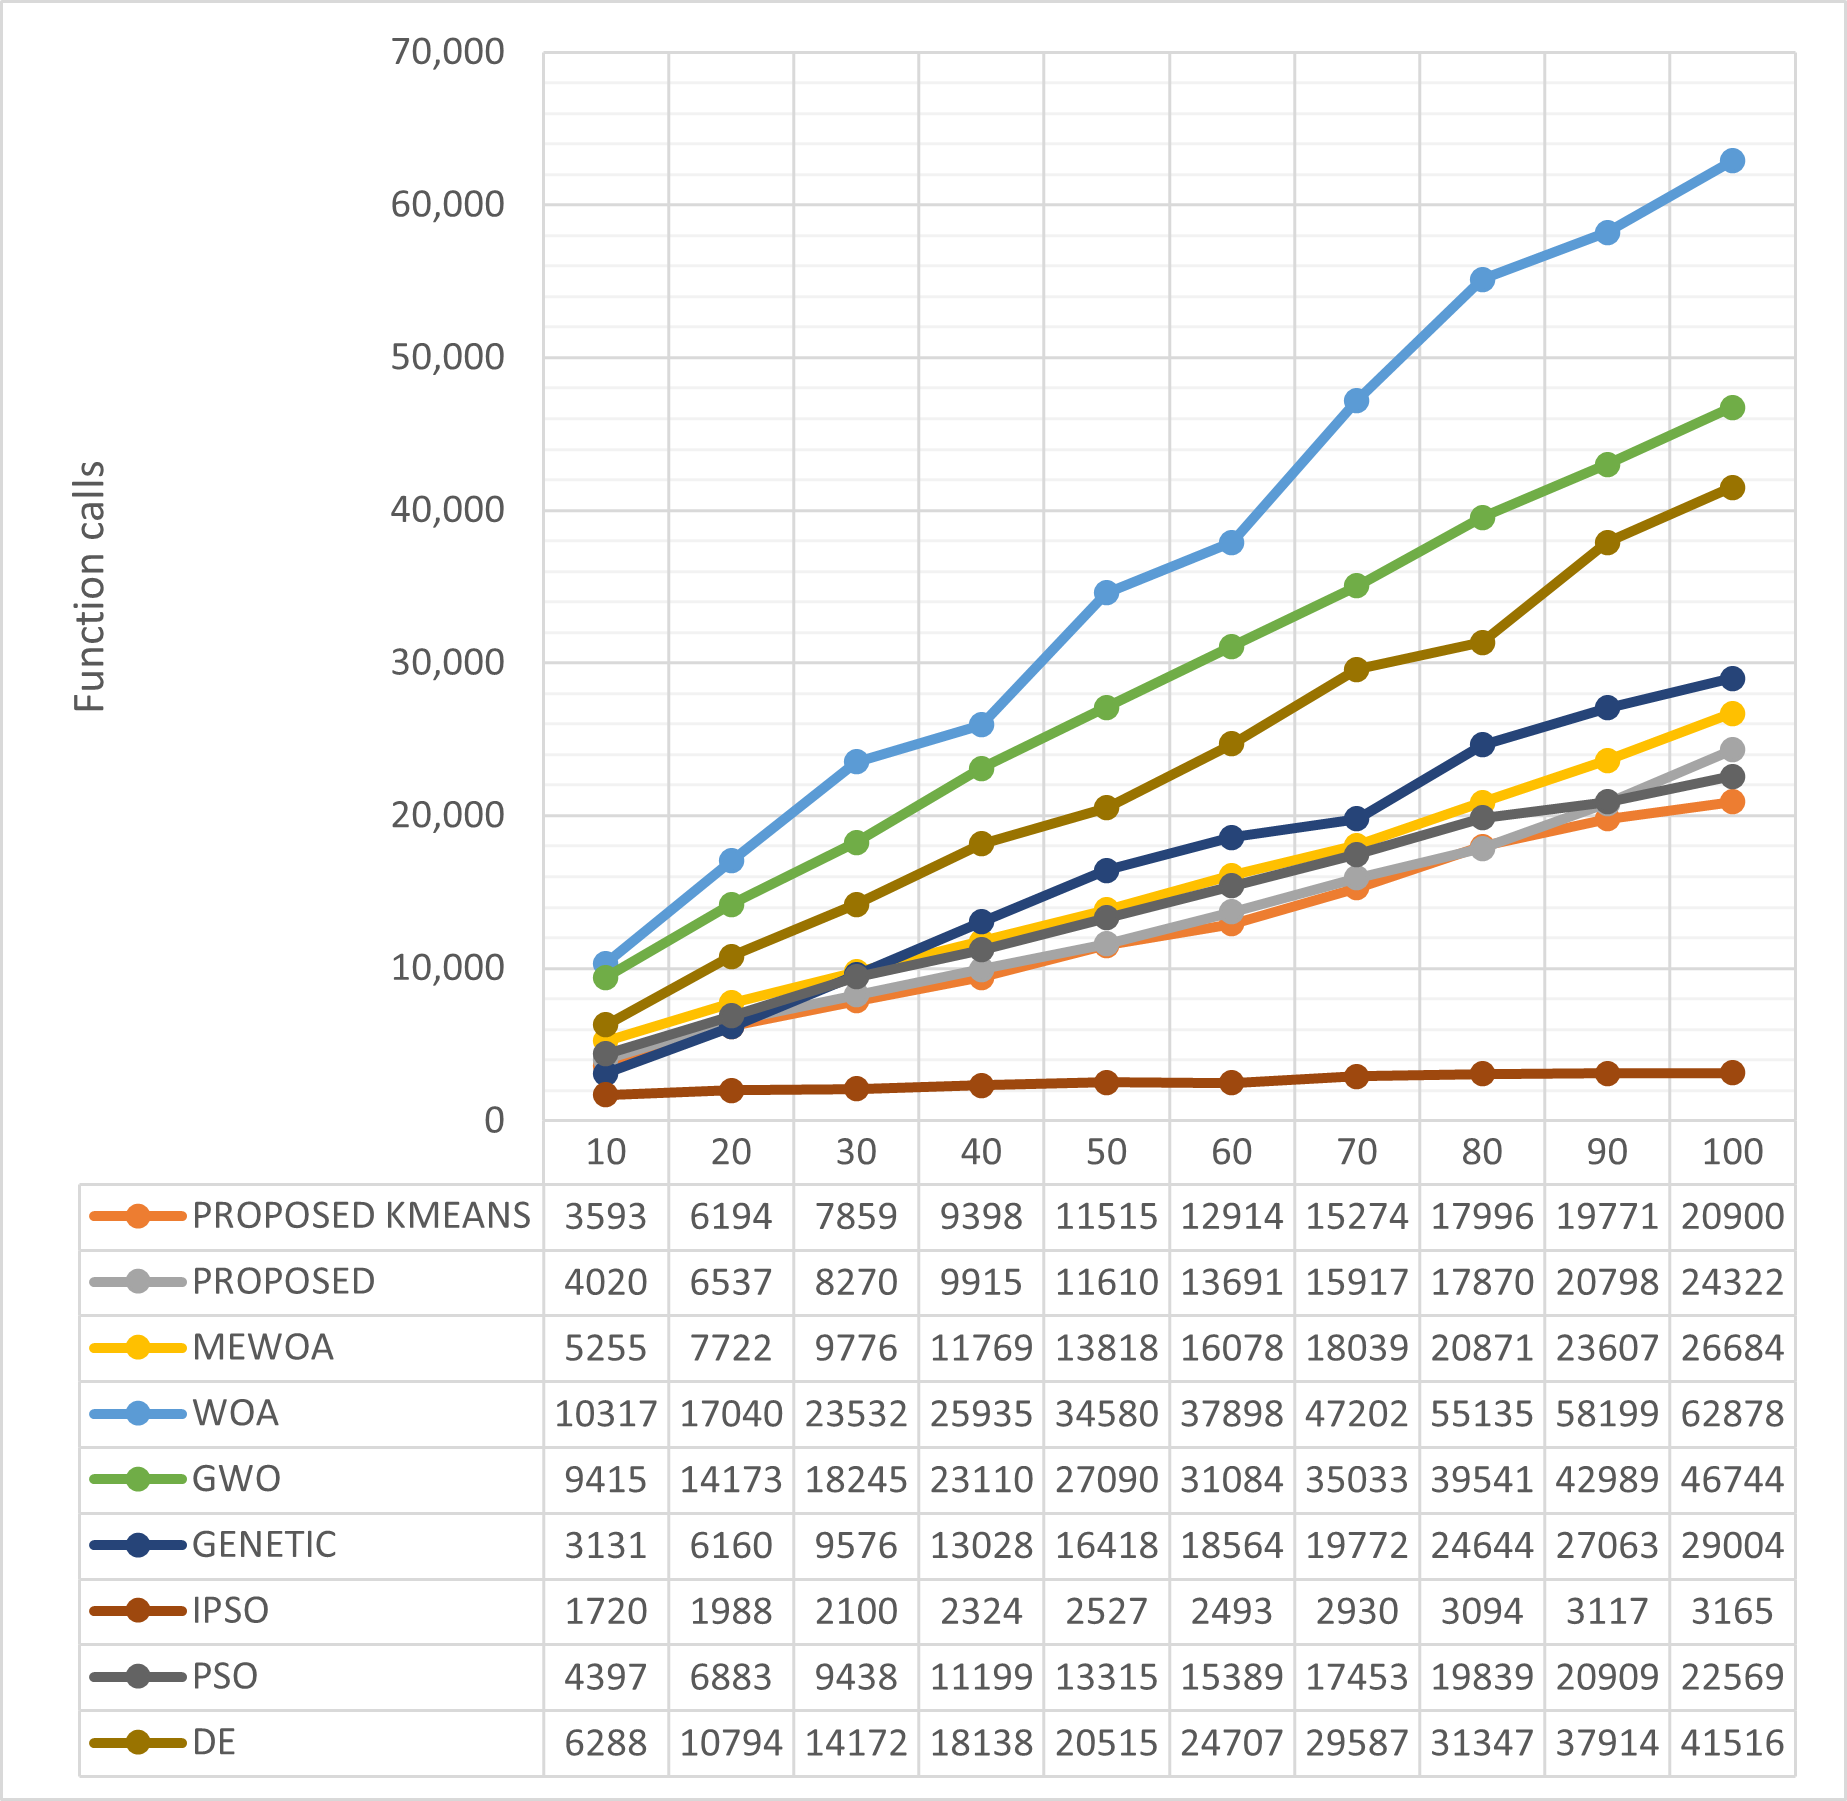
\includegraphics[scale=0.5]{new13}}\subfloat[Time comparison\label{fig:ELPTimes}]{\begin{centering}
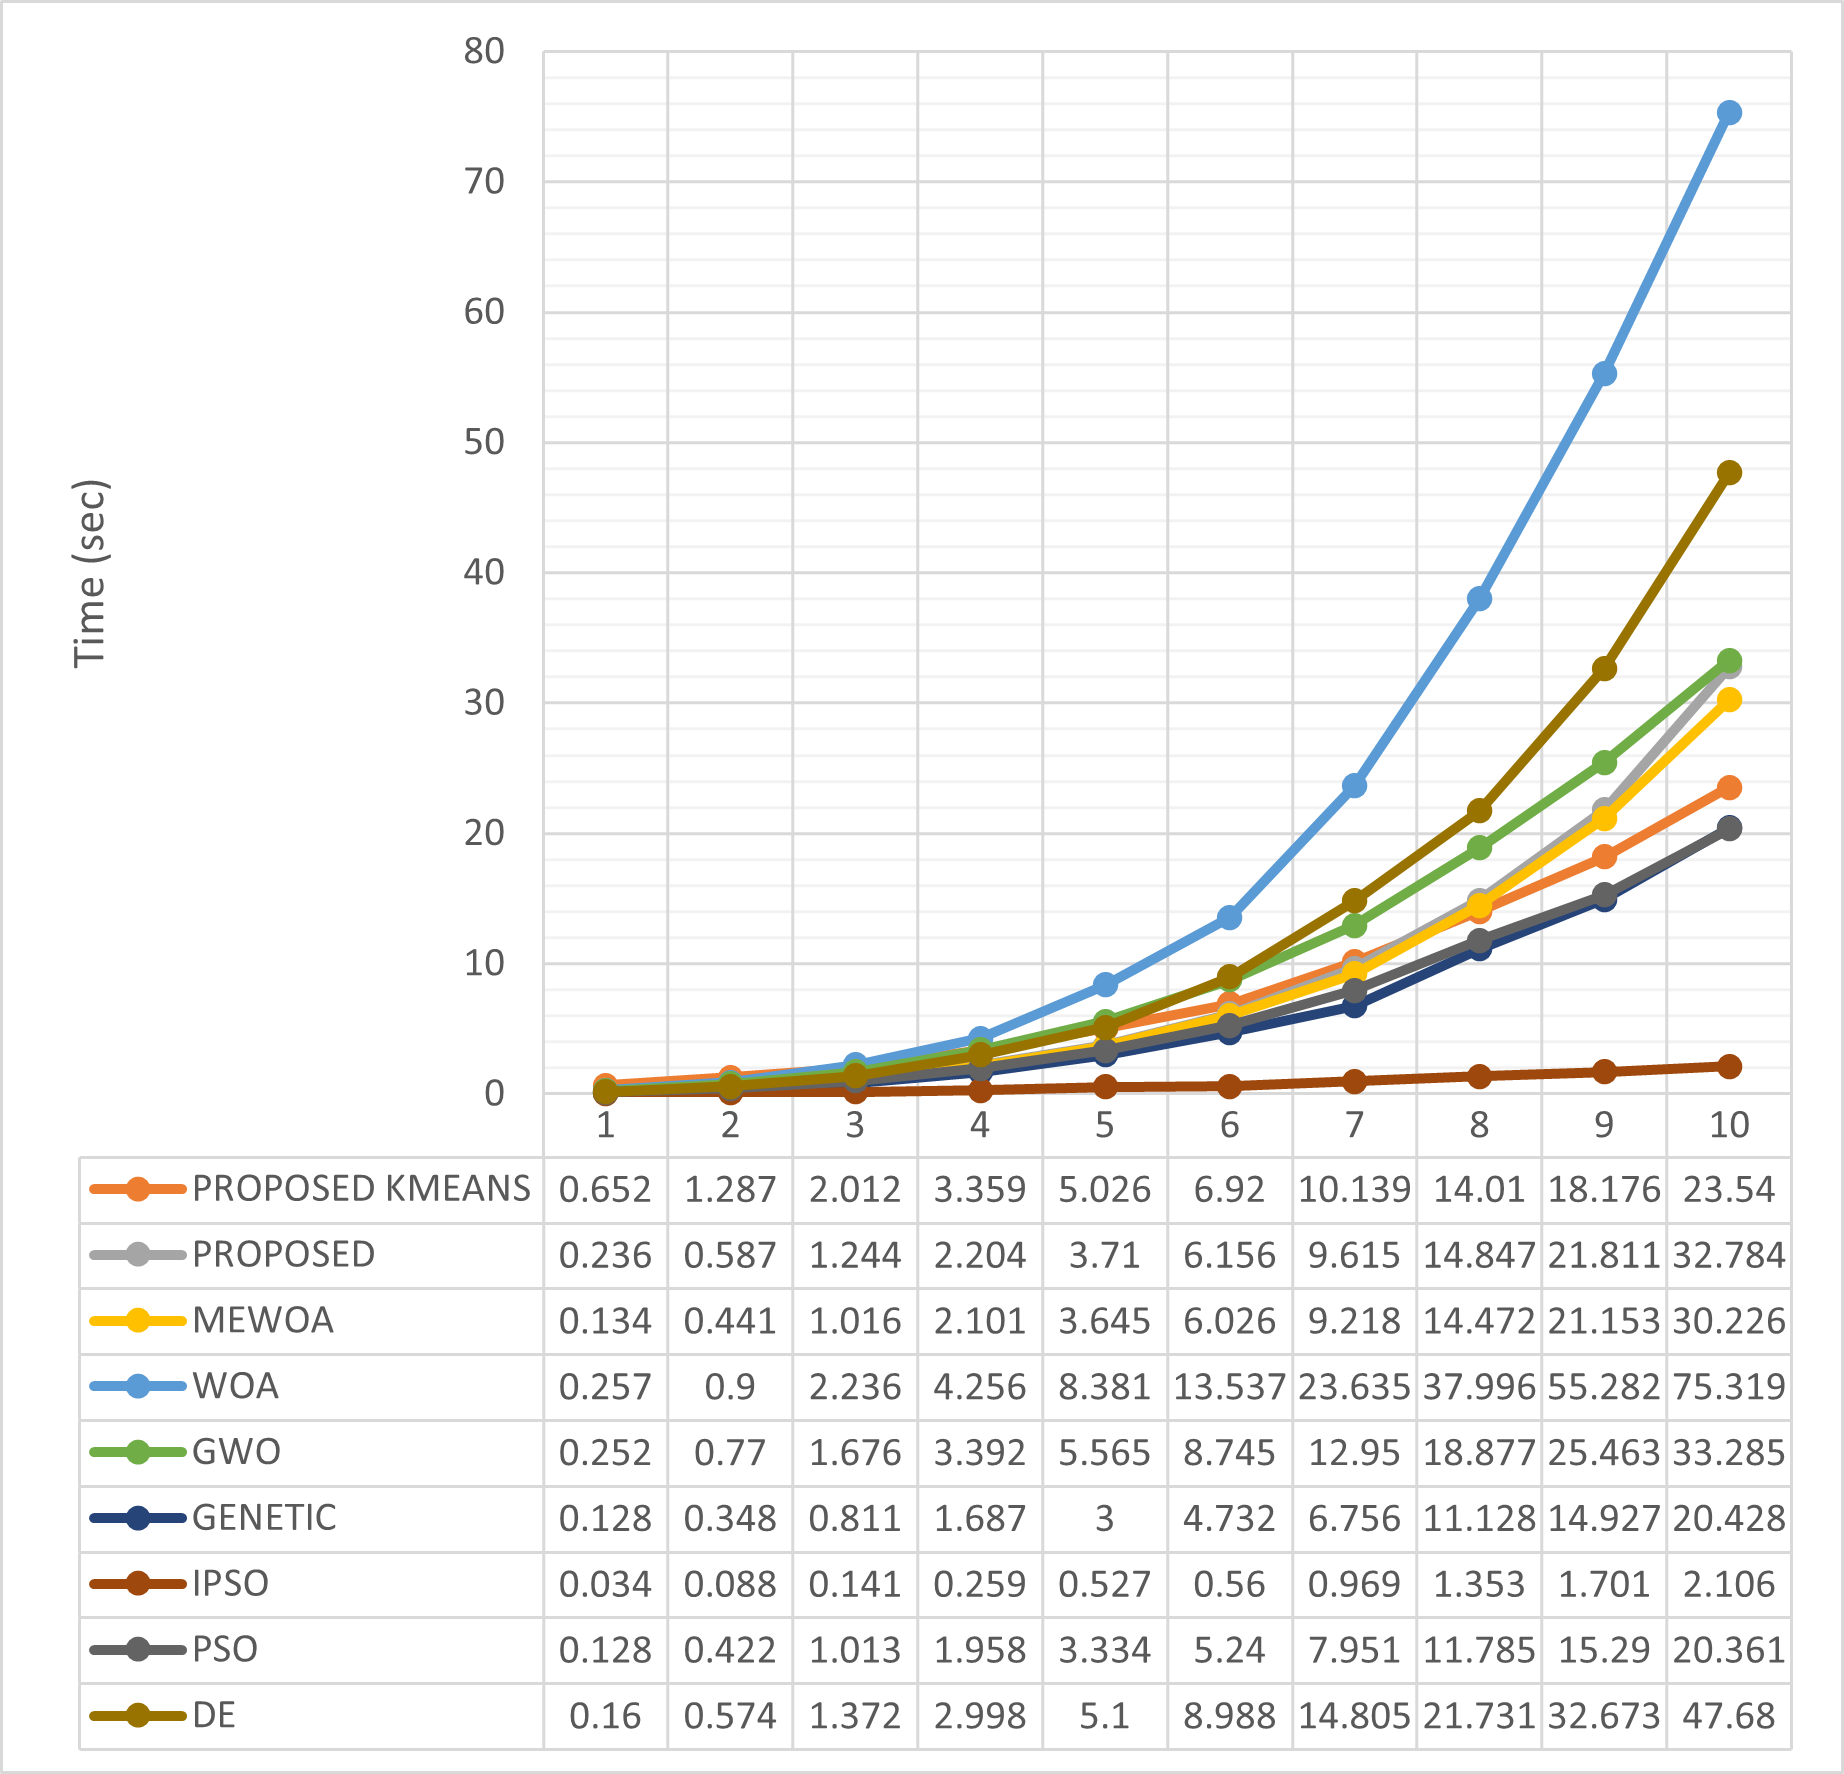
\includegraphics[scale=0.5]{new14}
\par\end{centering}
}\caption{Different variations of the ELP function of the proposed method with
other methods\protect\label{fig:ELP}}
\end{figure}
\par\end{center}

In each iteration of the algorithm, a trial point is calculated through
vector operations, similar to the process of optimization using differential
evolution. The main difference between the proposed method compared
to differential evolution lies in the fact that the samples for calculating
the trial point are selected from nearby regions of the initial distribution,
rather than being chosen randomly. However, the performance of the
two methods differs in their ability to find optimal solutions, as
shown in Figure \ref{eq:eq1}. In the case where the initial distribution
is created by the k-means algorithm, the performance increases by
36.3\%. The statistical analysis of the results in Figure \ref{fig:StatProposedVSOthers}
and Figure \ref{fig:proposedsVSDE} indicates that the proposed methods
(PROPOSED and PROPOSED+KMEANS) demonstrate statistically significantly
better performance than the DE method in most cases. The use of the
t-test confirms that these differences are not random but are due
to substantial improvements in the efficiency of the proposed methods.
The lower function call values show that the proposed methods lead
to faster convergence, and thus, better optimization performance.
The extraneous samples of Figure \ref{fig:compStatWithoutOutliers}
have been removed.
\begin{center}
\begin{figure}[H]
\centering{}\subfloat[Comparison of total function calls \label{fig:compTotal}]{\centering{}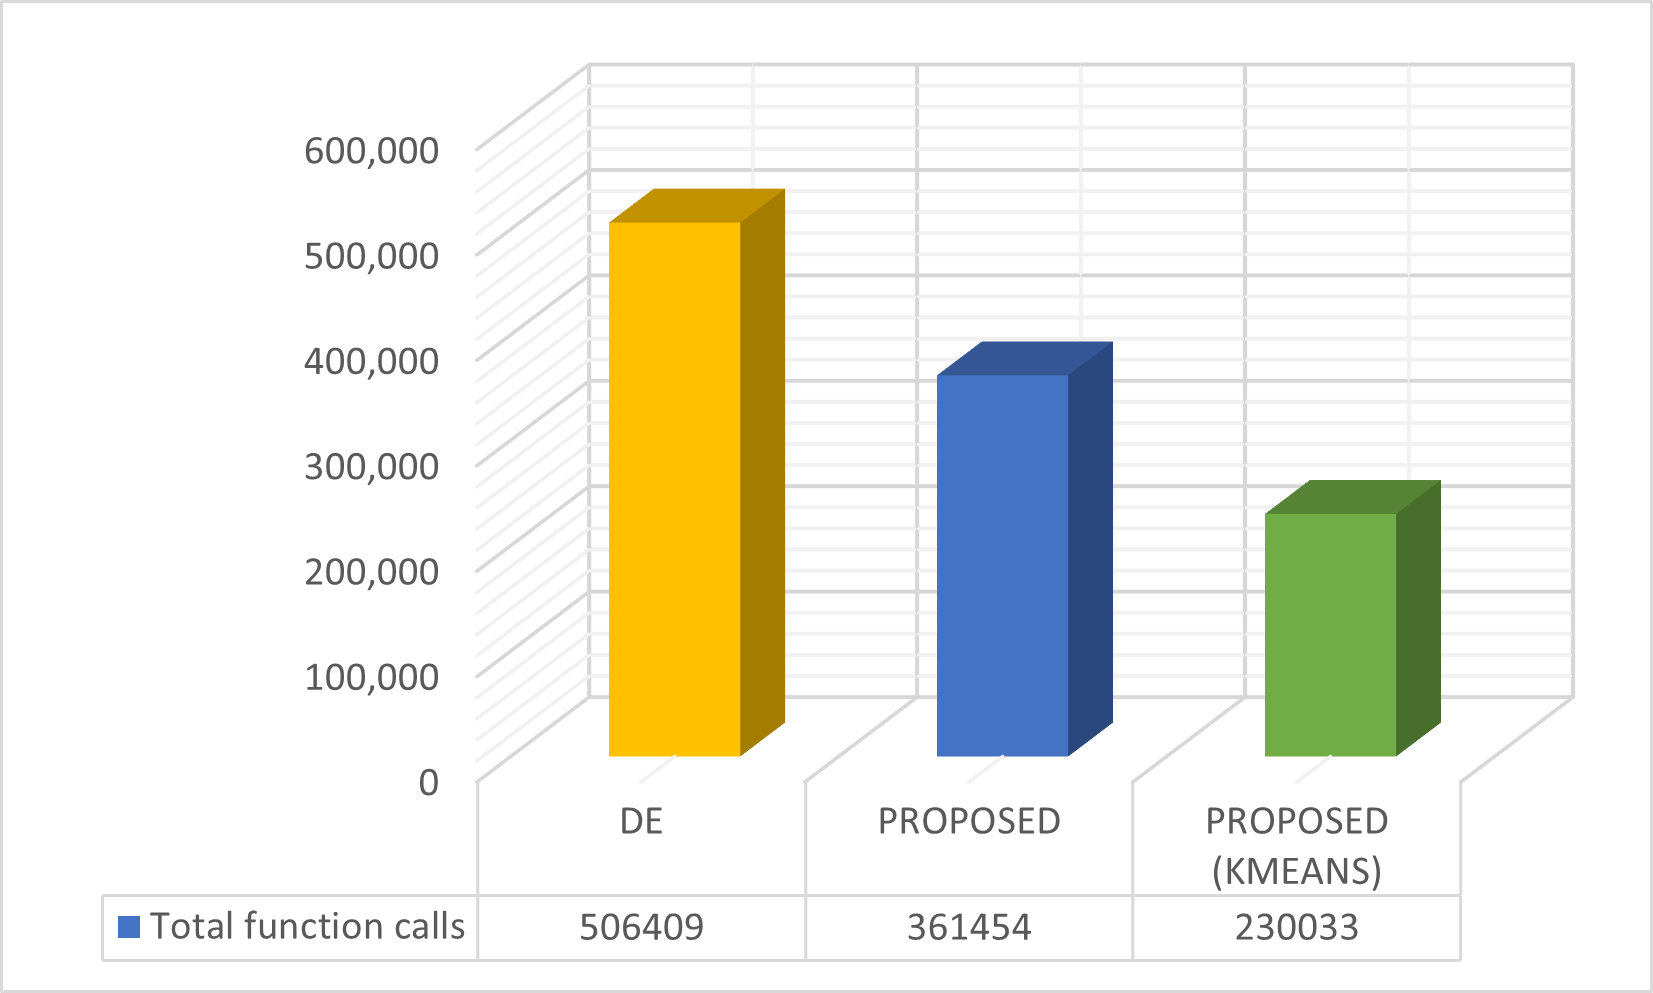
\includegraphics[scale=0.5]{new7}}\subfloat[Statistical comparison of total function calls\label{fig:compStatWithoutOutliers}]{\centering{}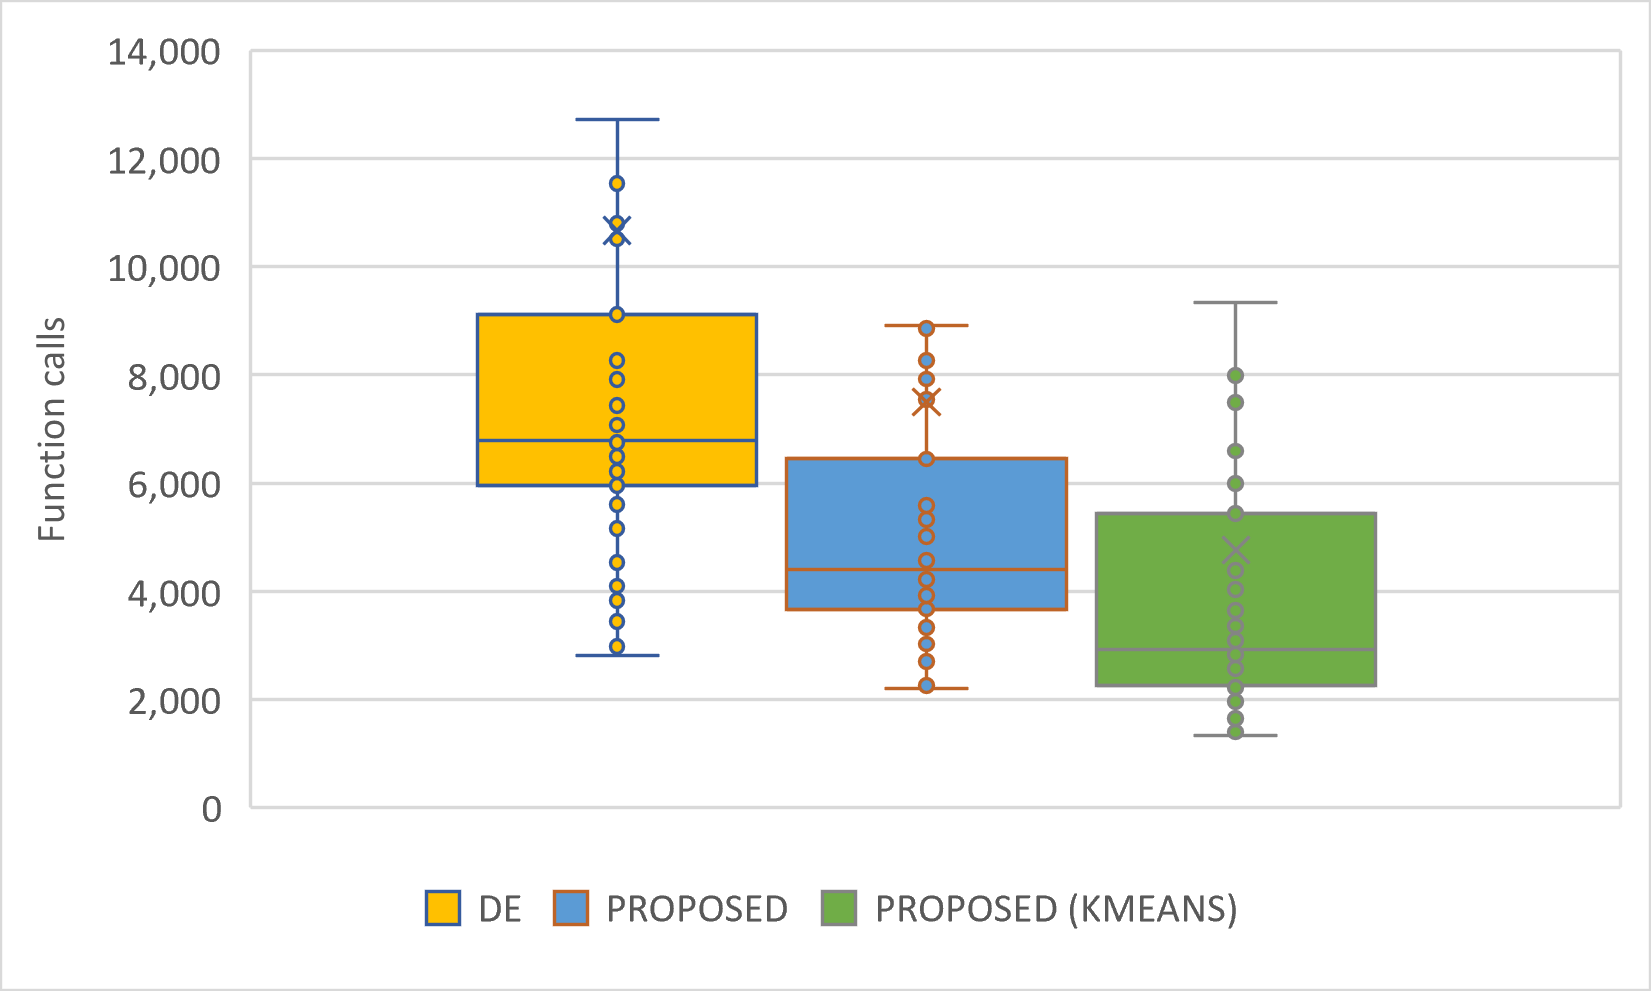
\includegraphics[scale=0.5]{new4}}\caption{Performance comparison of proposed methods against differential evolution:
Effect of K-Means algorithm on convergence.\protect\label{fig:proposedsVSDE}}
\end{figure}
\par\end{center}

\section{Conclusions\protect\label{sec:Conclusions}}

An innovative global optimization method has been proposed in this
research paper, which leverages techniques derived from well-established
optimization strategies. More specifically, the new method incorporates
genetic operators from Genetic Algorithms alongside the Linear Search
method to generate candidate solutions for the given objective functions.
These candidate solutions are then combined to create new solutions
utilizing approaches inspired by the Differential Evolution method.
To validate the effectiveness of this new optimization approach, a
comprehensive series of experiments were conducted on various problems
sourced from the existing literature. Additionally, numerical comparisons
were made with recognized global optimization techniques to provide
a clear benchmark. The results indicate that the proposed optimization
method exhibits significantly superior performance when compared to
alternative methods, particularly in terms of the number of calls
made to the objective function. Fewer calls to the objective function
suggest better overall efficiency, highlighting the proposed method's
ability to achieve optimal solutions with fewer evaluations. This
efficiency is particularly critical in scenarios where each function
call is computationally expensive. Statistical analysis, including
both the t-test and the Kruskal-Wallis test, confirm that the observed
differences in the number of calls between the proposed method and
other methods are statistically significant, with a p-value of less
than 0.05. This finding not only underscores the reduced resource
consumption of the proposed method but also affirms that it delivers
reliable results with enhanced efficiency. In summary, the proposed
method stands out in terms of efficiency when compared to other optimization
techniques, significantly decreasing the number of objective function
calls and optimizing overall computational cost. Potential enhancements
to the algorithm could involve identifying specific samples that contribute
more effectively to the discovery of the optimal solution. Furthermore,
since this method represents a novel approach to optimization, exploring
alternative termination criteria or varying the initial sample distributions
could lead to even greater performance improvements. By refining these
aspects, the method could further bolster its efficiency and effectiveness
in solving complex optimization problems.

\vspace{6pt}


\authorcontributions{The conceptualization of the idea and the design of the methodology,
as well as the supervision of the technical aspects related to the
software, were undertaken by V.C., I.G.T., and G.K. The experiments
were conducted using various datasets, and the comparative results
were presented by V.C., G.K. and A.M.G. The statistical analysis was
carried out by V.C. The manuscript was prepared by G.K. and the other
authors. All authors have reviewed and approved the final published
version.}

\funding{No external funding was received for this research.}

\institutionalreview{Not applicable.}

\informedconsent{Not applicable. }

\institutionalreview{Not applicable.}

\acknowledgments{This research has been financed by the European Union: Next Generation
EU through the Program Greece 2.0 National Recovery and Resilience
Plan, under the call RESEARCH--CREATE--INNOVATE, project name “iCREW:
Intelligent small craft simulator for advanced crew training using
Virtual Reality techniques” (project code: TAEDK-06195).}

\conflictsofinterest{The authors declare no conflicts of interest.}

\conflictsofinterest{No conflicts of interest are declared by the authors.}

\appendixtitles{no}

\reftitle{References}
\begin{thebibliography}{999}
\bibitem{go_math1}Carrizosa, E., Molero-Río, C., \& Romero Morales,
D. (2021). Mathematical optimization in classification and regression
trees. Top, 29(1), 5-33.

\bibitem{go_physics1}Stilck França, D., \& Garcia-Patron, R. (2021).
Limitations of optimization algorithms on noisy quantum devices. Nature
Physics, 17(11), 1221-1227.

\bibitem{go_chem1}Zhang, J., \& Glezakou, V. A. (2021). Global optimization
of chemical cluster structures: Methods, applications, and challenges.
International Journal of Quantum Chemistry, 121(7), e26553.

\bibitem{medicine}Houssein, E. H., Hosney, M. E., Mohamed, W. M.,
Ali, A. A., \& Younis, E. M. (2023). Fuzzy-based hunger games search
algorithm for global optimization and feature selection using medical
data. Neural Computing and Applications, 35(7), 5251-5275.

\bibitem{go_bio2}Hesami, M., \& Jones, A. M. P. (2020). Application
of artificial intelligence models and optimization algorithms in plant
cell and tissue culture. Applied Microbiology and Biotechnology, 104(22),
9449-9485.

\bibitem{go_agri1}Filip, M., Zoubek, T., Bumbalek, R., Cerny, P.,
Batista, C. E., Olsan, P., ... \& Findura, P. (2020). Advanced computational
methods for agriculture machinery movement optimization with applications
in sugarcane production. Agriculture, 10(10), 434.

\bibitem{go_econ1}Alirahmi, S. M., Mousavi, S. B., Razmi, A. R.,
\& Ahmadi, P. (2021). A comprehensive techno-economic analysis and
multi-criteria optimization of a compressed air energy storage (CAES)
hybridized with solar and desalination units. Energy Conversion and
Management, 236, 114053.

\bibitem{go_determ1}Shezan, S. A., Ishraque, M. F., Shafiullah, G.
M., Kamwa, I., Paul, L. C., Muyeen, S. M., ... \& Kumar, P. P. (2023).
Optimization and control of solar-wind islanded hybrid microgrid by
using heuristic and deterministic optimization algorithms and fuzzy
logic controller. Energy reports, 10, 3272-3288.

\bibitem{stohastic}Hsieh, Y. P., Karimi Jaghargh, M. R., Krause,
A., \& Mertikopoulos, P. (2024). Riemannian stochastic optimization
methods avoid strict saddle points. Advances in Neural Information
Processing Systems, 36.

\bibitem{interval1}Villanueva, F. R., \& de Oliveira, V. A. (2022).
Necessary optimality conditions for interval optimization problems
with functional and abstract constraints. Journal of Optimization
Theory and Applications, 194(3), 896-923.

\bibitem{Sergeyev}Sergeyev, Y. D., Kvasov, D. E., \& Mukhametzhanov,
M. S. (2018). On the efficiency of nature-inspired metaheuristics
in expensive global optimization with limited budget. Scientific reports,
8(1), 453.

\bibitem{genetic3}Charilogis, V., Tsoulos, I. G., \& Stavrou, V.
N. (2023). An Intelligent Technique for Initial Distribution of Genetic
Algorithms. Axioms, 12(10), 980.

\bibitem{diffe1}Deng, W., Shang, S., Cai, X., Zhao, H., Song, Y.,
\& Xu, J. (2021). An improved differential evolution algorithm and
its application in optimization problem. Soft Computing, 25, 5277-5298.

\bibitem{pso_major}Shami, T. M., El-Saleh, A. A., Alswaitti, M.,
Al-Tashi, Q., Summakieh, M. A., \& Mirjalili, S. (2022). Particle
swarm optimization: A comprehensive survey. Ieee Access, 10, 10031-10061.

\bibitem{aco1}Rokbani, N., Kumar, R., Abraham, A., Alimi, A. M.,
Long, H. V., Priyadarshini, I., \& Son, L. H. (2021). Bi-heuristic
ant colony optimization-based approaches for traveling salesman problem.
Soft Computing, 25, 3775-3794.

\bibitem{fish}Pourpanah, F., Wang, R., Lim, C. P., Wang, X. Z., \&
Yazdani, D. (2023). A review of artificial fish swarm algorithms:
Recent advances and applications. Artificial Intelligence Review,
56(3), 1867-1903.

\bibitem{dolphin}Kareem, S. W., Mohammed, A. S., \& Khoshabaa, F.
S. (2023). Novel nature-inspired meta-heuristic optimization algorithm
based on hybrid dolphin and sparrow optimization. International Journal
of Nonlinear Analysis and Applications, 14(1), 355-373. 

\bibitem{WOA}Nadimi-Shahraki, M. H., Zamani, H., Asghari Varzaneh,
Z., \& Mirjalili, S. (2023). A systematic review of the whale optimization
algorithm: theoretical foundation, improvements, and hybridizations.
Archives of Computational Methods in Engineering, 30(7), 4113-4159.

\bibitem{key-7}Lalwani, S., Sharma, H., Satapathy, S. C., Deep, K.,
\& Bansal, J. C. (2019). A survey on parallel particle swarm optimization
algorithms. Arabian Journal for Science and Engineering, 44, 2899-2923.

\bibitem{gpu1}Hussain, M. M., \& Fujimoto, N. (2020). GPU-based parallel
multi-objective particle swarm optimization for large swarms and high
dimensional problems. Parallel Computing, 92, 102589.

\bibitem{holland}Eshelman, L. J. (2018). Genetic algorithms. In Evolutionary
Computation 1 (pp. 102-118). CRC Press.

\bibitem{ga_problem1}Hervis Santana, Y., Martinez Alonso, R., Guillen
Nieto, G., Martens, L., Joseph, W., \& Plets, D. (2022). Indoor genetic
algorithm-based 5G network planning using a machine learning model
for path loss estimation. Applied Sciences, 12(8), 3923.

\bibitem{key-33}Liu, X., Jiang, D., Tao, B., Jiang, G., Sun, Y.,
Kong, J., ... \& Chen, B. (2022). Genetic algorithm-based trajectory
optimization for digital twin robots. Frontiers in Bioengineering
and Biotechnology, 9, 793782.

\bibitem{key-35}Liu, K., Deng, B., Shen, Q., Yang, J., \& Li, Y.
(2022). Optimization based on genetic algorithms on energy conservation
potential of a high speed SI engine fueled with butanol--gasoline\LyXZeroWidthSpace{}
blends. Energy Reports, 8, 69-80.

\bibitem{key-29}MirRokni, M. K. S. M. (2017). Applying genetic algorithm
in architecture and neural network training. International Journal
of Computer Science and Network Security IJCSN, 17(6), 118.

\bibitem{de_symmetry1}Li, Y. H., Wang, J. Q., Wang, X. J., Zhao,
Y. L., Lu, X. H., \& Liu, D. L. (2017). Community detection based
on differential evolution using social spider optimization. Symmetry,
9(9), 183.

\bibitem{de_problem1}Maulik, U., \& Saha, I. (2010). Automatic fuzzy
clustering using modified differential evolution for image classification.
IEEE transactions on Geoscience and Remote sensing, 48(9), 3503-3510.

\bibitem{key-37}Vivekanandan, T., \& Iyengar, N. C. S. N. (2017).
Optimal feature selection using a modified differential evolution
algorithm and its effectiveness for prediction of heart disease. Computers
in biology and medicine, 90, 125-136.

\bibitem{de_deep1}Wu, T., Li, X., Zhou, D., Li, N., \& Shi, J. (2021).
Differential evolution based layer-wise weight pruning for compressing
deep neural networks. Sensors, 21(3), 880.

\bibitem{go_local2}Badem, H., Basturk, A., Caliskan, A., \& Yuksel,
M. E. (2018). A new hybrid optimization method combining artificial
bee colony and limited-memory BFGS algorithms for efficient numerical
optimization. Applied Soft Computing, 70, 826-844.

\bibitem{hybrid1}Li, S., Tan, M., Tsang, I. W., \& Kwok, J. T. Y.
(2011). A hybrid PSO-BFGS strategy for global optimization of multimodal
functions. IEEE Transactions on Systems, Man, and Cybernetics, Part
B (Cybernetics), 41(4), 1003-1014.

\bibitem{hybrid2}Andalib Sahnehsaraei, M., Mahmoodabadi, M. J., Taherkhorsandi,
M., Castillo-Villar, K. K., \& Mortazavi Yazdi, S. M. (2015). A hybrid
global optimization algorithm: particle swarm optimization in association
with a genetic algorithm. Complex System Modelling and Control Through
Intelligent Soft Computations, 45-86.

\bibitem{armijo}Huang, P., Huang, H. Z., \& Huang, T. (2019). A novel
algorithm for structural reliability analysis based on finite step
length and Armijo line search. Applied Sciences, 9(12), 2546.

\bibitem[(2022)]{charilogis}Charilogis, V., \& Tsoulos, I. G. (2022).
Toward an ideal particle swarm optimizer for multidimensional functions.
Information, 13(5), 217.

\bibitem{gwo}Mirjalili, S., Mirjalili, S. M., \& Lewis, A. (2014).
Grey wolf optimizer. Advances in engineering software, 69, 46-61.

\bibitem{kmeansNew}Ahmed, M., Seraj, R., \& Islam, S. M. S. (2020).
The k-means algorithm: A comprehensive survey and performance evaluation.
Electronics, 9(8), 1295.

\bibitem[(2002)]{bfgs} Dai, Y. H. (2002). Convergence properties
of the BFGS algoritm. SIAM Journal on Optimization, 13(3), 693-701.

\bibitem{Gaviano} Gaviano, M., Kvasov, D. E., Lera, D., \& Sergeyev,
Y. D. (2003). Algorithm 829: Software for generation of classes of
test functions with known local and global minima for global optimization.
ACM Transactions on Mathematical Software (TOMS), 29(4), 469-480.

\bibitem{Lennard} Jones, J. E. (1924). On the determination of molecular
fields.---II. From the equation of state of a gas. Proceedings of
the Royal Society of London. Series A, Containing Papers of a Mathematical
and Physical Character, 106(738), 463-477.

\bibitem{Zabinsky}Zabinsky, Z. B., Graesser, D. L., Tuttle, M. E.,
\& Kim, G. I. (1992). Global optimization of composite laminates using
improving hit and run. In Recent advances in global optimization (pp.
343-368).

\bibitem{Ali1}Ali, M. M., Khompatraporn, C., \& Zabinsky, Z. B. (2005).
A numerical evaluation of several stochastic algorithms on selected
continuous global optimization test problems. Journal of global optimization,
31, 635-672.

\bibitem{Floudas1}Floudas, C. A., Pardalos, P. M., Adjiman, C., Esposito,
W. R., Gümüs, Z. H., Harding, S. T., ... \& Schweiger, C. A. (2013).
Handbook of test problems in local and global optimization (Vol. 33).
Springer Science \& Business Media.

\bibitem{key-6}Storn, R. (1996, June). On the usage of differential
evolution for function optimization. In Proceedings of North American
fuzzy information processing (pp. 519-523). Ieee.

\bibitem[(2023)]{memoa}Shen, Y., Zhang, C., Gharehchopogh, F. S.,
\& Mirjalili, S. (2023). An improved whale optimization algorithm
based on multi-population evolution for global optimization and engineering
design problems. Expert Systems with Applications, 215, 119269\textbf{.}

\bibitem{powell}Powell, M. J. D. (1989). A tolerant algorithm for
linearly constrained optimization calculations. Mathematical Programming,
45, 547-566.

\end{thebibliography}

\end{document}
